\documentclass[final]{article}

% if you need to pass options to natbib, use, e.g.:
% \PassOptionsToPackage{numbers, compress}{natbib}
% before loading nips_2017
%
% to avoid loading the natbib package, add option nonatbib:
% \usepackage[nonatbib]{nips_2017}

\usepackage{nips_2017}

% to compile a camera-ready version, add the [final] option, e.g.:
% \usepackage[final]{nips_2017}

\usepackage[utf8]{inputenc} % allow utf-8 input
\usepackage[T1]{fontenc}    % use 8-bit T1 fonts
\usepackage{hyperref}       % hyperlinks
\usepackage{url}            % simple URL typesetting
\usepackage{booktabs}       % professional-quality tables
\usepackage{amsfonts}       % blackboard math symbols
\usepackage{nicefrac}       % compact symbols for 1/2, etc.
\usepackage{microtype}      % microtypography
\usepackage{amsmath}
\usepackage{graphicx}
\usepackage{booktabs}
\DeclareMathOperator*{\Motimes}{\text{\raisebox{0.25ex}{\scalebox{0.8}{$\bigotimes$}}}}

% \usepackage{lmodern}

\usepackage{graphicx}
\usepackage{caption}
\usepackage{subcaption}
\usepackage{tikz}
\usepackage{float}
\usetikzlibrary{shapes, arrows}

\title{Predicting Stock Trends with Fourier Analysis}

% The \author macro works with any number of authors. There are two
% commands used to separate the names and addresses of multiple
% authors: \And and \AND.
%
% Using \And between authors leaves it to LaTeX to determine where to
% break the lines. Using \AND forces a line break at that point. So,
% if LaTeX puts 3 of 4 authors names on the first line, and the last
% on the second line, try using \AND instead of \And before the third
% author name.

\author{
  Forest Kobayashi \\
  Department of Mathematics\\
  Harvey Mudd College\\
  Claremont, CA 91711 \\
  \texttt{fkobayash@hmc.edu} \\
  %% examples of more authors
  \And
  Jacky Lee \\
  Department of Mathematics\\
  Department of Computer Science \\
  Harvey Mudd College \\
  Claremont, CA 91711 \\
  \texttt{jaclee@hmc.edu}
}

\begin{document}
% \nipsfinalcopy is no longer used

\maketitle

\begin{abstract}
  Stock data is very difficult to analyze using classical methods, in
  large part due to heavy involvement of humans in stock pricing. In
  this paper, we examine a new approach to analyzing time-series stock
  data, particularly in the context of grouping correlated stocks.
\end{abstract}

\section{Introduction}

Here is a rough table of contents for our paper, so that the reader
has a rough idea of where we'll be going:
\begin{enumerate}
  \item Background and Motivation (challenges to modelling stock data)
  \item Long-term goal for the model / ideal model architecture
  \item Classification and Prediction
  \item Results
  \item Conclusion
\end{enumerate}

\section{Background and Motivation}

There are many reasons why predicting stock prices is difficult, but
for our model today, we will focus on just two:
\begin{enumerate}
  \item The behavior of a given stock is influenced by hundreds of
    hidden variables --- e.g., the current state of geopolitics,
    governmental fiscal policies (for instance, the US Treasury
    interest rate), the performance of stocks in various other
    markets, etc. Hence, the price of a stock at any given moment is
    an emergent phenomenon, influenced by many small movements of
    markets around the world. Further, these connections themselves
    are in a constant state of flux --- as the market evolves,
    technology improves, and policies are rewritten, the weight each
    of these variables has in influencing pricing will wax and wane.
  \item With the exception of some forms of algo trading, most trading
    strategies are being created and implemented by humans. That is,
    often humans are the ones who perform analysis of market
    information, and make decisions based off the findings. But humans
    are not naturally predisposed to rigorous quantitative analysis,
    and hence markets do not always behave rationally. As an example,
    consider \texttt{Bitcoin}.\footnote{Citation: Gary Evans} Thus,
    an accurate financial model will need to have some method of
    predicting human psychology.
\end{enumerate}

Using modern machine learning techniques, it is possible to control
for some effects of (2) by using previous stock data. However,
less work has been done to model the effects of (1). So, for today's
model, we will focus on methods of preprocessing time series stock
data so as to control for some of the effects of (1).

% Stock prices can be influenced by many factors such as other stock
% prices, anticipation of capital gains or losses, global politics,
% earnings reports, and etc. These factors may each have a different
% weighting on the stock depending on time and which stock is being
% analyzed in question. For example, earnings reports might have
% significantly more impact on stock prices immediately after release as
% opposed to two months after the report comes out. Another example
% would be that global politics might influence the stock price of
% \textbf{LMT} (Lockheed Martin), an aerospace and defense company, more
% than the stock price of \textbf{BKC} (Burger King), a fast food
% restaurant chain.

% Ultimately, humans are the ones who choose to buy, sell, or short
% these stocks based on some analysis, usually not completely
% comprehensive, of the factors they observe. Since humans are often
% unaware or unable to analyze all these competing factors at once,
% their decisions are often unpredictable or at least very difficult to
% predict. As such, predicting the price of stocks by modeling these
% interactions between stock price factors and humans is difficult and
% unwise. Therefore, we have decided to perform stock analysis by only
% analyzing past stock trends. This approach, although loses out on a
% lot of information, is computationally less demanding and easier to
% find data for performing analysis.

\section{The Model}

\subsection{Goals}

Our ultimate goal is to be able to use past stock data to train our
model. Then given some stock trend data for some stock, use our model
to predict the upcoming trends and return a vector of decisions. An
example of the output is shown below.

\[
  \mathbf{y} = \Bigl<P_{sell}(\mathbf{x}), P_{nothing}(\mathbf{x}),
  P_{buy}(\mathbf{x})\Bigr>
\]

Here, $P_{buy}(\mathbf{x})$ represents how confident the model is in
recommending the user to buy the stock. Similarly,
$P_{sell}(\mathbf{x})$ represents selling the stock,
$P_{short}(\mathbf{x})$ represents shorting the stock, and
$P_{nothing}(\mathbf{x})$ represents doing nothing. All these
probabilities should sum to 1.

In order to reach this sort of conclusion, we want our model to
compensate for the effects of (1) in a clever way. In traditional
stock trading practices, there are a few guidelines that are used for
similar determinations:
\begin{enumerate}
  \item Someimtes industries follow trends together. For instance, if
    we see a price drop in one oil stock, we might expect to see drops
    in other oil stocks.
  \item When interest rates go up, yield-bearing financial assests
    increase in value, while the value of equity stocks might
    decrease.
  \item If an earnings report reveals that a stock overestimated its
    expected profits, the value of the stock will decrease.
  \item In times of high uncertainty, money might be pulled out of
    equity assets and moved to yield-bearing financial assets. Hence,
    stock prices might go down.
  \item Bad PR can result in a temporary dip in stock pricing.
\end{enumerate}

These are external factors that cannot be determined purely from the
stock data itself. Often, most of this information comes from news
outlets, press releases, and other media-sharing forums. So, we need
our model to perform the following:
\begin{enumerate}
  \item Scrape real-time text data from news websites, financial
    websites, and (possibly) academic journals in the case that we're
    looking at something like a technology stock.
  \item Perform some sort of Natural Language Processing and Sentiment
    Analysis to determine how this information might affect the market
    if / when it becomes widely publicized.
  \item Somehow combine this information with time-series stock data
    to make a prediction of how the market might behave in the short
    and long term.
  \item Make a trading decision based on this information.
\end{enumerate}
We propose the following prototype model.

\subsection{Prototype Architecture}

Before we get into it, we want to stress that this is a heavily
compartmentalized model we built to try and capture how we want
information to flow and be processed. In reality, we'd want to
collapse some of the nodes into a single process, and remove some of
the overall complexity to make training easier. We are not saying this
would be easy to implement and / or train without significant
computing power, just that this model could accomplish what we desire.
\begin{figure}[H]
  \centering
    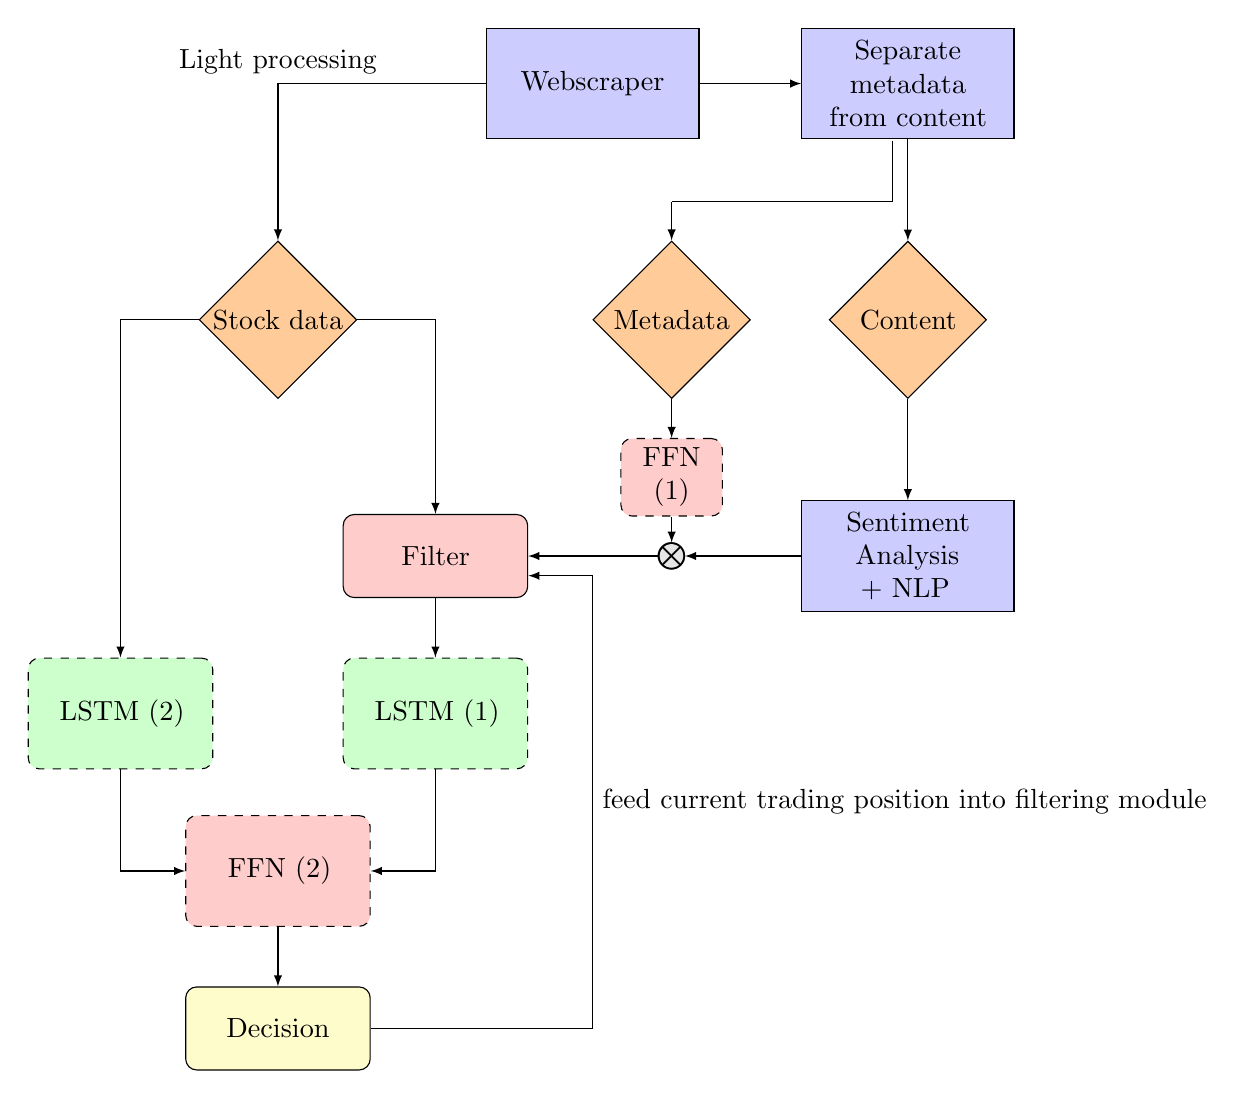
\begin{tikzpicture}[node distance = 2cm, auto]
      \tikzstyle{data} = [
        diamond,
        draw,
        fill=orange!40,
        text width = 5em,
        text badly centered,
        node distance = 3cm,
        inner sep = 0pt
      ]

      \tikzstyle{code} = [
        rectangle,
        draw,
        fill=blue!20,
        text width=7em,
        text centered,
        minimum height=4em
      ]

      \tikzstyle{network} = [
        rectangle,
        draw,
        dashed,
        fill=green!20,
        text width = 6em,
        text centered,
        rounded corners,
        minimum height = 4em
      ]

      \tikzstyle{feedforward} = [
        rectangle,
        draw,
        dashed,
        fill=red!20,
        text width = 6em,
        text centered,
        rounded corners,
        minimum height = 4em
      ]

      \tikzstyle{filter} = [
        draw,
        rectangle,
        fill=red!20,
        text width = 6em,
        text centered,
        minimum height=3em,
        rounded corners
      ]

      \tikzstyle{decision} = [
        draw,
        rectangle,
        fill=yellow!20,
        text width = 6em,
        text centered,
        minimum height=3em,
        rounded corners
      ]

      \tikzstyle{otimes} = [
        draw,
        circle,
        fill=gray!20,
        text centered,
        inner sep = -2pt
      ]

      \node[code] (webscraper) at (0,6) {Webscraper};
      \node[data] (time series) at (-4,3) {Stock data};
      \node[code] (parser) at (4,6) {Separate metadata from content};
      \node[data] (text) at (4,3) {Content};
      \node[code] (processer) at (4,0) {Sentiment Analysis + NLP};
      \node[filter] (filter) at (-2,0) {Filter};
      \node[network] (lstm1) at (-2,-2) {LSTM (1)};
      \node[network] (lstm2) at (-6,-2) {LSTM (2)};
      \node[feedforward] (feedforward) at (-4,-4) {FFN (2)};
      \node[decision] (decision) at (-4,-6) {Decision};
      \node[data] (metadata) at (1,3) {Metadata};
      \node[draw, rectangle, fill=red!20, text width = 3em, text
      centered, minimum height = 2em, rounded corners, dashed]
      (ffilter) at (1,1) {FFN (1)};
      \node[otimes] (otimes) at (1,0) {$\bigotimes$};



      \draw[-latex] (webscraper) -| (time series) node[midway, above]
      {Light processing};
      \draw[-latex] (webscraper) -- (parser);
      \draw[-latex] (parser) -- (text);
      \draw[-latex] (text) -- (processer) node[midway, right] {};
      \draw (3.8,5.27) -- (3.8,4.5) -- (1,4.5);
      \draw[-latex] (1, 4.5) -- (metadata);
      \draw[-latex] (time series) -| (filter);
      \draw[-latex] (filter) -- (lstm1);
      \draw[-latex] (processer) -- (otimes);
      \draw[-latex] (otimes) -- (filter);
      \draw[-latex] (ffilter) -- (otimes);
      \draw[-latex] (metadata) -- (ffilter);
      \draw[-latex] (time series) -| (lstm2);
      \draw[-latex] (lstm2) |- (feedforward);
      \draw[-latex] (lstm1) |- (feedforward);
      \draw[-latex] (feedforward) -- (decision);
      \draw (decision) -- (0,-6) -- (0,-.25) node[midway, right] {feed
      current trading position into filtering module};
      \draw[-latex] (0,-.25) -- (-.82,-.25) node[midway, right] {};
    \end{tikzpicture}
  \caption{Model overview}
  \label{fig:goal}
\end{figure}
Of course, as we just said, this is not the optimal architecture. But
let's walk through the rationale before discounting it entirely:
\begin{enumerate}
  \item We scrape two types of data: time series stock data, as well
    as news / financial / academic articles.
  \item To preprocess the stock data, we extract the time series and
    convert it into an array, abstracting the data in some manner so
    that we can make all inputs the same size. We embed the stock
    symbol itself with a word vector, so that the network can learn to
    differentiate behaviors of different stocks. This will also be
    employed in the subsequent filtering stage.
  \item To preprocess the text data, we first separate out the
    metadata from the content, and clean things like html tags out of
    the body (depending on how we're doing the scraping). We perform
    Natural Language Processing methods on the input data (e.g.,
    sentiment analysis), to try and quantify whether the article
    represents good news or bad news for some stock.
  \item We feed the metadata into a feedforward network that is
    trained to determine the bias of the source from which each datum
    was obtained. The $\tanh()$ function will be used, because we
    want to be able to ``flip'' the input from some organization if
    it consistently predicts the opposite of what actually happens.
  \item At the $\otimes$ junction, we do elementwise multiplication of
    the output from FFN (1) with the output from our sentiment
    analysis of our articles. These will then be sorted by the stocks
    they apply to, and we will take the harmonic mean of these values
    to obtain a single predictive value for the behavior of the stock
    in the near future.
  \item Next, we feed this into a filter, which will choose a few
    families of stocks for LSTM (1) to focus on. The filter might
    include some neural architecture itself, and will incorporate
    information about the network's current assests.
  \item We take the most significant stocks output by the filter,
    along with some sentiment data about it, and feed this heavily
    into LSTM (1), which will be a relatively deep network.
  \item Simultaneously, we feed the unprocessed stock data (without
    selecting a noteworthy subset) into LSTM (2), which will be a much
    shallower network, the idea being that LSTM (2) might pick up on
    noteworthy trends that the news articles missed.
  \item Finally, this is input into a small feedforward network that
    aggregates the processed and unprocessed inputs, and returns
    decisions to buy, sell, short, or do nothing with respect to some
    particular stock. The process is then repeated, and ideall the
    network would turn a profit.
\end{enumerate}

For today's paper, we focused on the filtering stage. In particular,
we wanted to identify ways of classifying families of noteworthy
stocks that LSTM (1) could make predictions on, and identify abstract
relationships between pricing of various stocks. Our rationale was
this: most of the other components of the diagram are famous problems
that others have already performed lost of work on. That is, using
LSTMs to predict stock pricing is, for the most part, a solved
problem. Implementations and hyperparameters may differ, of course,
but underneath, the structure of the model is largely the same. We saw
the filtering process as the component we could perhaps make
advancments on.

\section{Methods}

\subsection{Data Scraping}

We gathered intraday data for three randomly-selected S\&P 500 stocks
using the Alpha Vantage API
(\url{https://github.com/RomelTorres/alpha_vantage}). A portion of the
data for one stock is shown below.

\begin{verbatim}
                     1. open  2. high   3. low   4. close  5. volume
date
2018-05-08 09:30:00  1058.54  1058.54  1055.00  1055.1600    26407.0
2018-05-08 09:31:00  1054.99  1058.16  1054.99  1056.9248     6384.0
2018-05-08 09:32:00  1057.41  1058.95  1057.41  1058.5700     7160.0
2018-05-08 09:33:00  1058.30  1058.64  1056.93  1058.6400     6448.0
2018-05-08 09:34:00  1058.80  1060.00  1058.50  1059.9600     5548.0
\end{verbatim}

For each stock, we computed the arithmetic mean of the high and low as
a heuristic for summarizing the price of the stock during that minute.
For our minimal working prototype, we decided to ignore the data for
the volume of trading, the open price, and the close price, since
stock prices vary quite a bit and we felt that the high and low prices
would be sufficient in giving us an estimate of how the stock was
preforming at that moment in time. However, when composing a more
polished model in the future, we will be sure to include this
information.

\subsection{Data Windowing}

We then analyzed the data by running a sliding window of 20 data points (20
minutes) across the prices, with each window having a large overlap with the
previous (to make the data smoother). Specifically, each consecutive window was
only shifted by 2 minutes. This windowed data was analyzed in two different ways.

The windows were fitted with polynomials and the coefficients were then
extracted for Fourier analysis. The frequency and amplitude information gained
from the Fourier analysis was then used for classification via a k-means
clustering algorithm.

Linear regression was also performed on the windows and the slopes were
extracted for analysis using a Markov model. Recent slope data was used to
predict upcoming slopes in the hopes of predicting upcoming stock trends.

\subsection{Clustering with Fourier Coefficients}

\subsubsection{Polynomial Fitting on Windowed Data}

With the windowed data, we fit a quintic polynomial to each window. Three such
polynomials fitted to three consecutive windows are shown below.

\begin{figure}[H]
  \centering
  \begin{subfigure}{.3\textwidth}
    \centering
    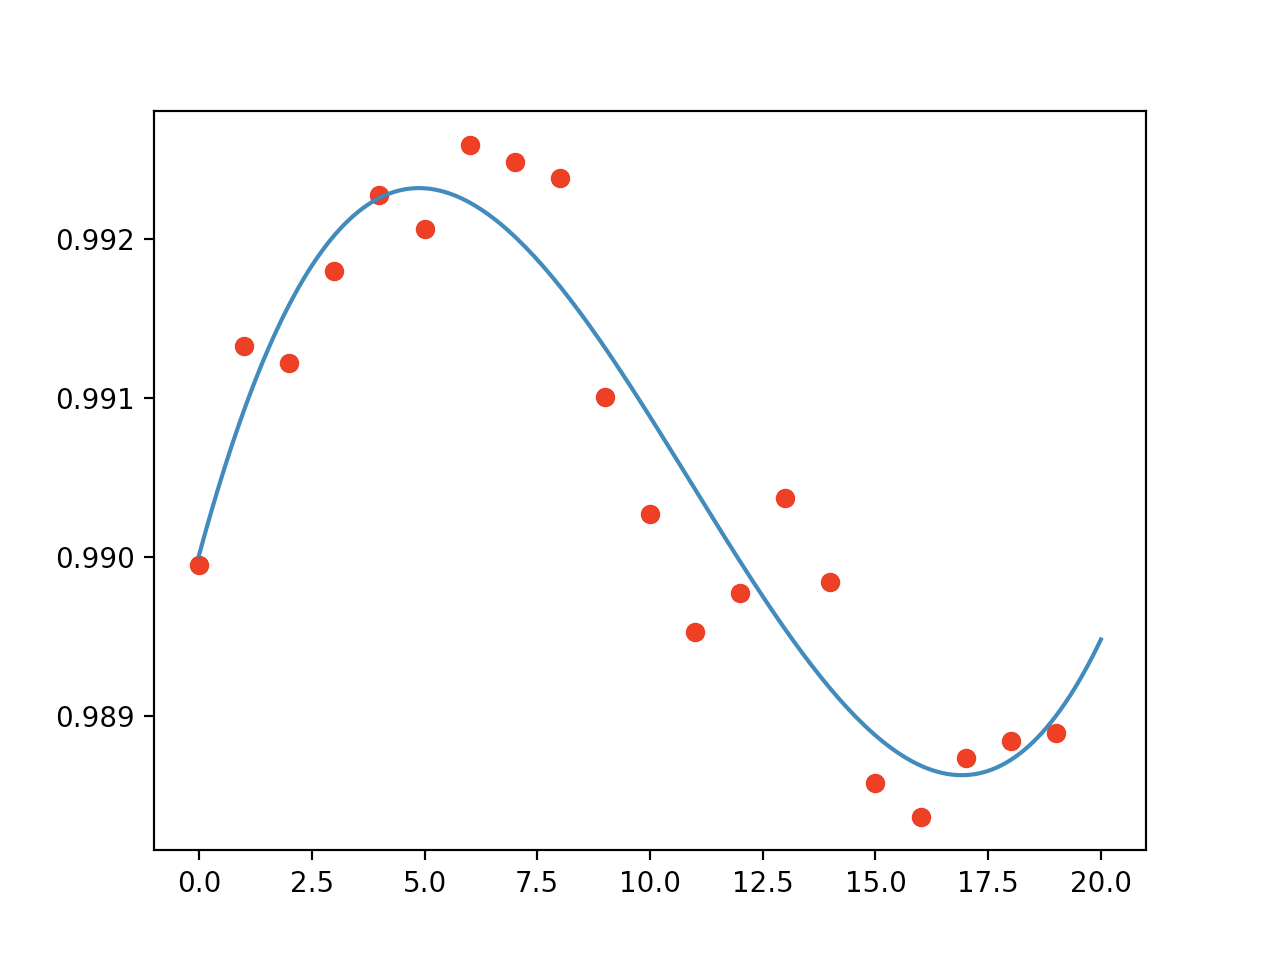
\includegraphics[width=\linewidth]{img/sliding1}
  \end{subfigure}
  \begin{subfigure}{.3\textwidth}
    \centering
    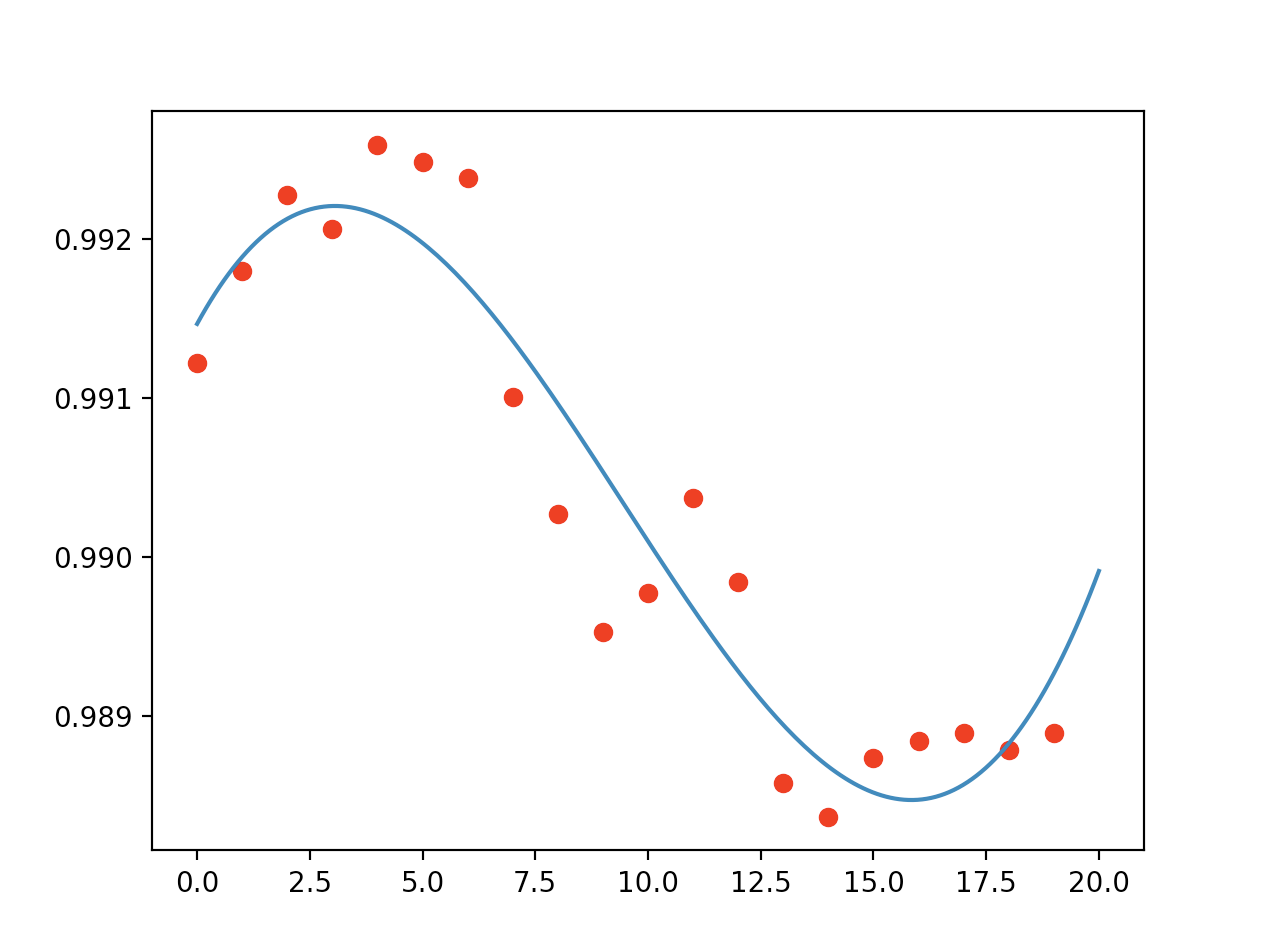
\includegraphics[width=\linewidth]{img/sliding2}
  \end{subfigure}
  \begin{subfigure}{.3\textwidth}
    \centering
    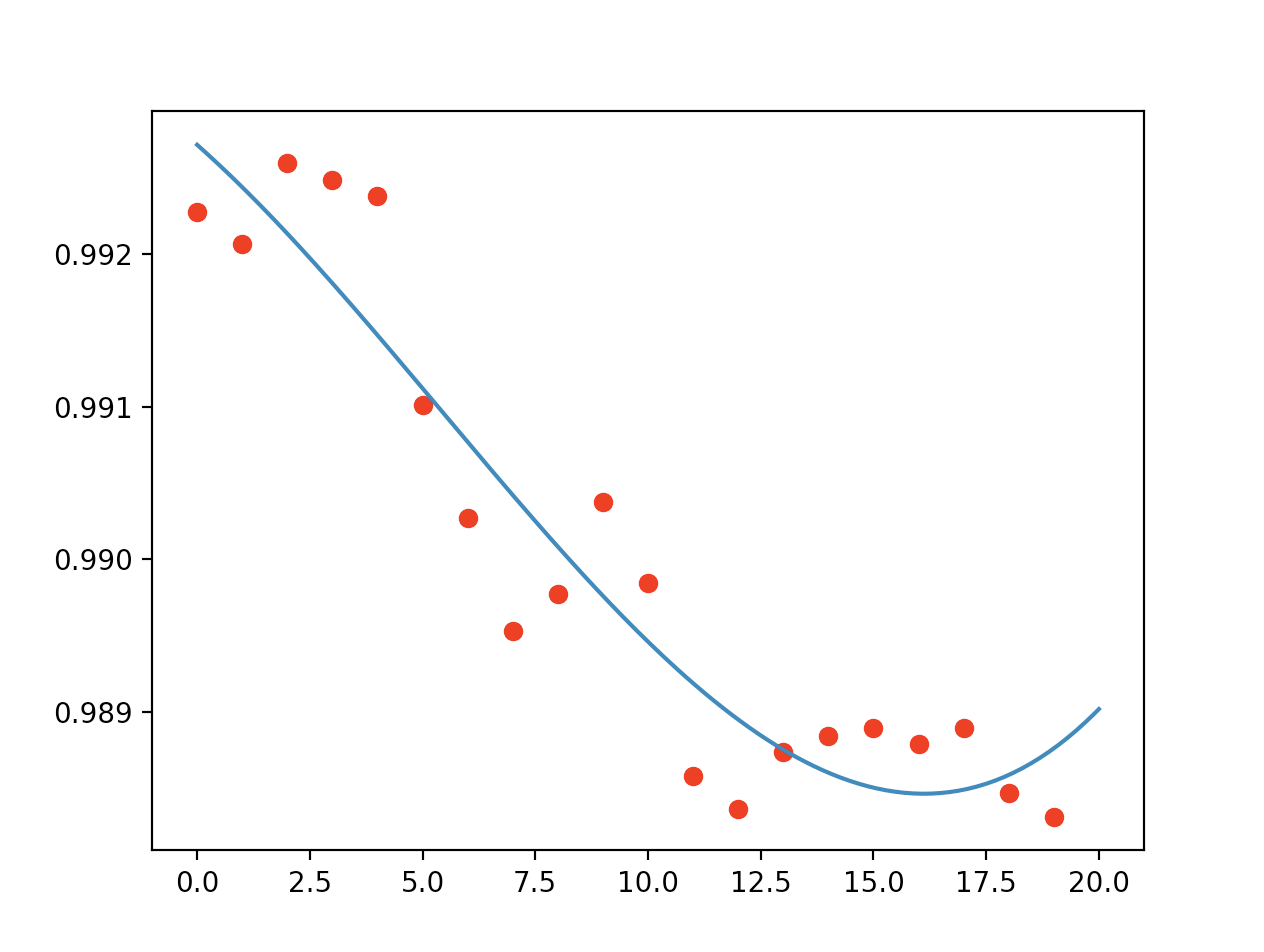
\includegraphics[width=\linewidth]{img/sliding3}
  \end{subfigure}
  \caption{Sliding windows of data fitted with polynomials}
  \label{fig:sliding}
\end{figure}

% TODO: justify a quintic

\subsubsection{Visualizing the Coefficients}

After performing this sliding window analysis on each of the stocks,
we then plotted the coefficients of our polynomial fits in
$\mathbb{R}^3$ to visualize our data. We were hoping that we'd gain
insight by examining the structure of these trajectories through time.
Some examples are shown below.

\begin{figure}[H]
  \centering
  \begin{subfigure}{.45\textwidth}
    \centering
    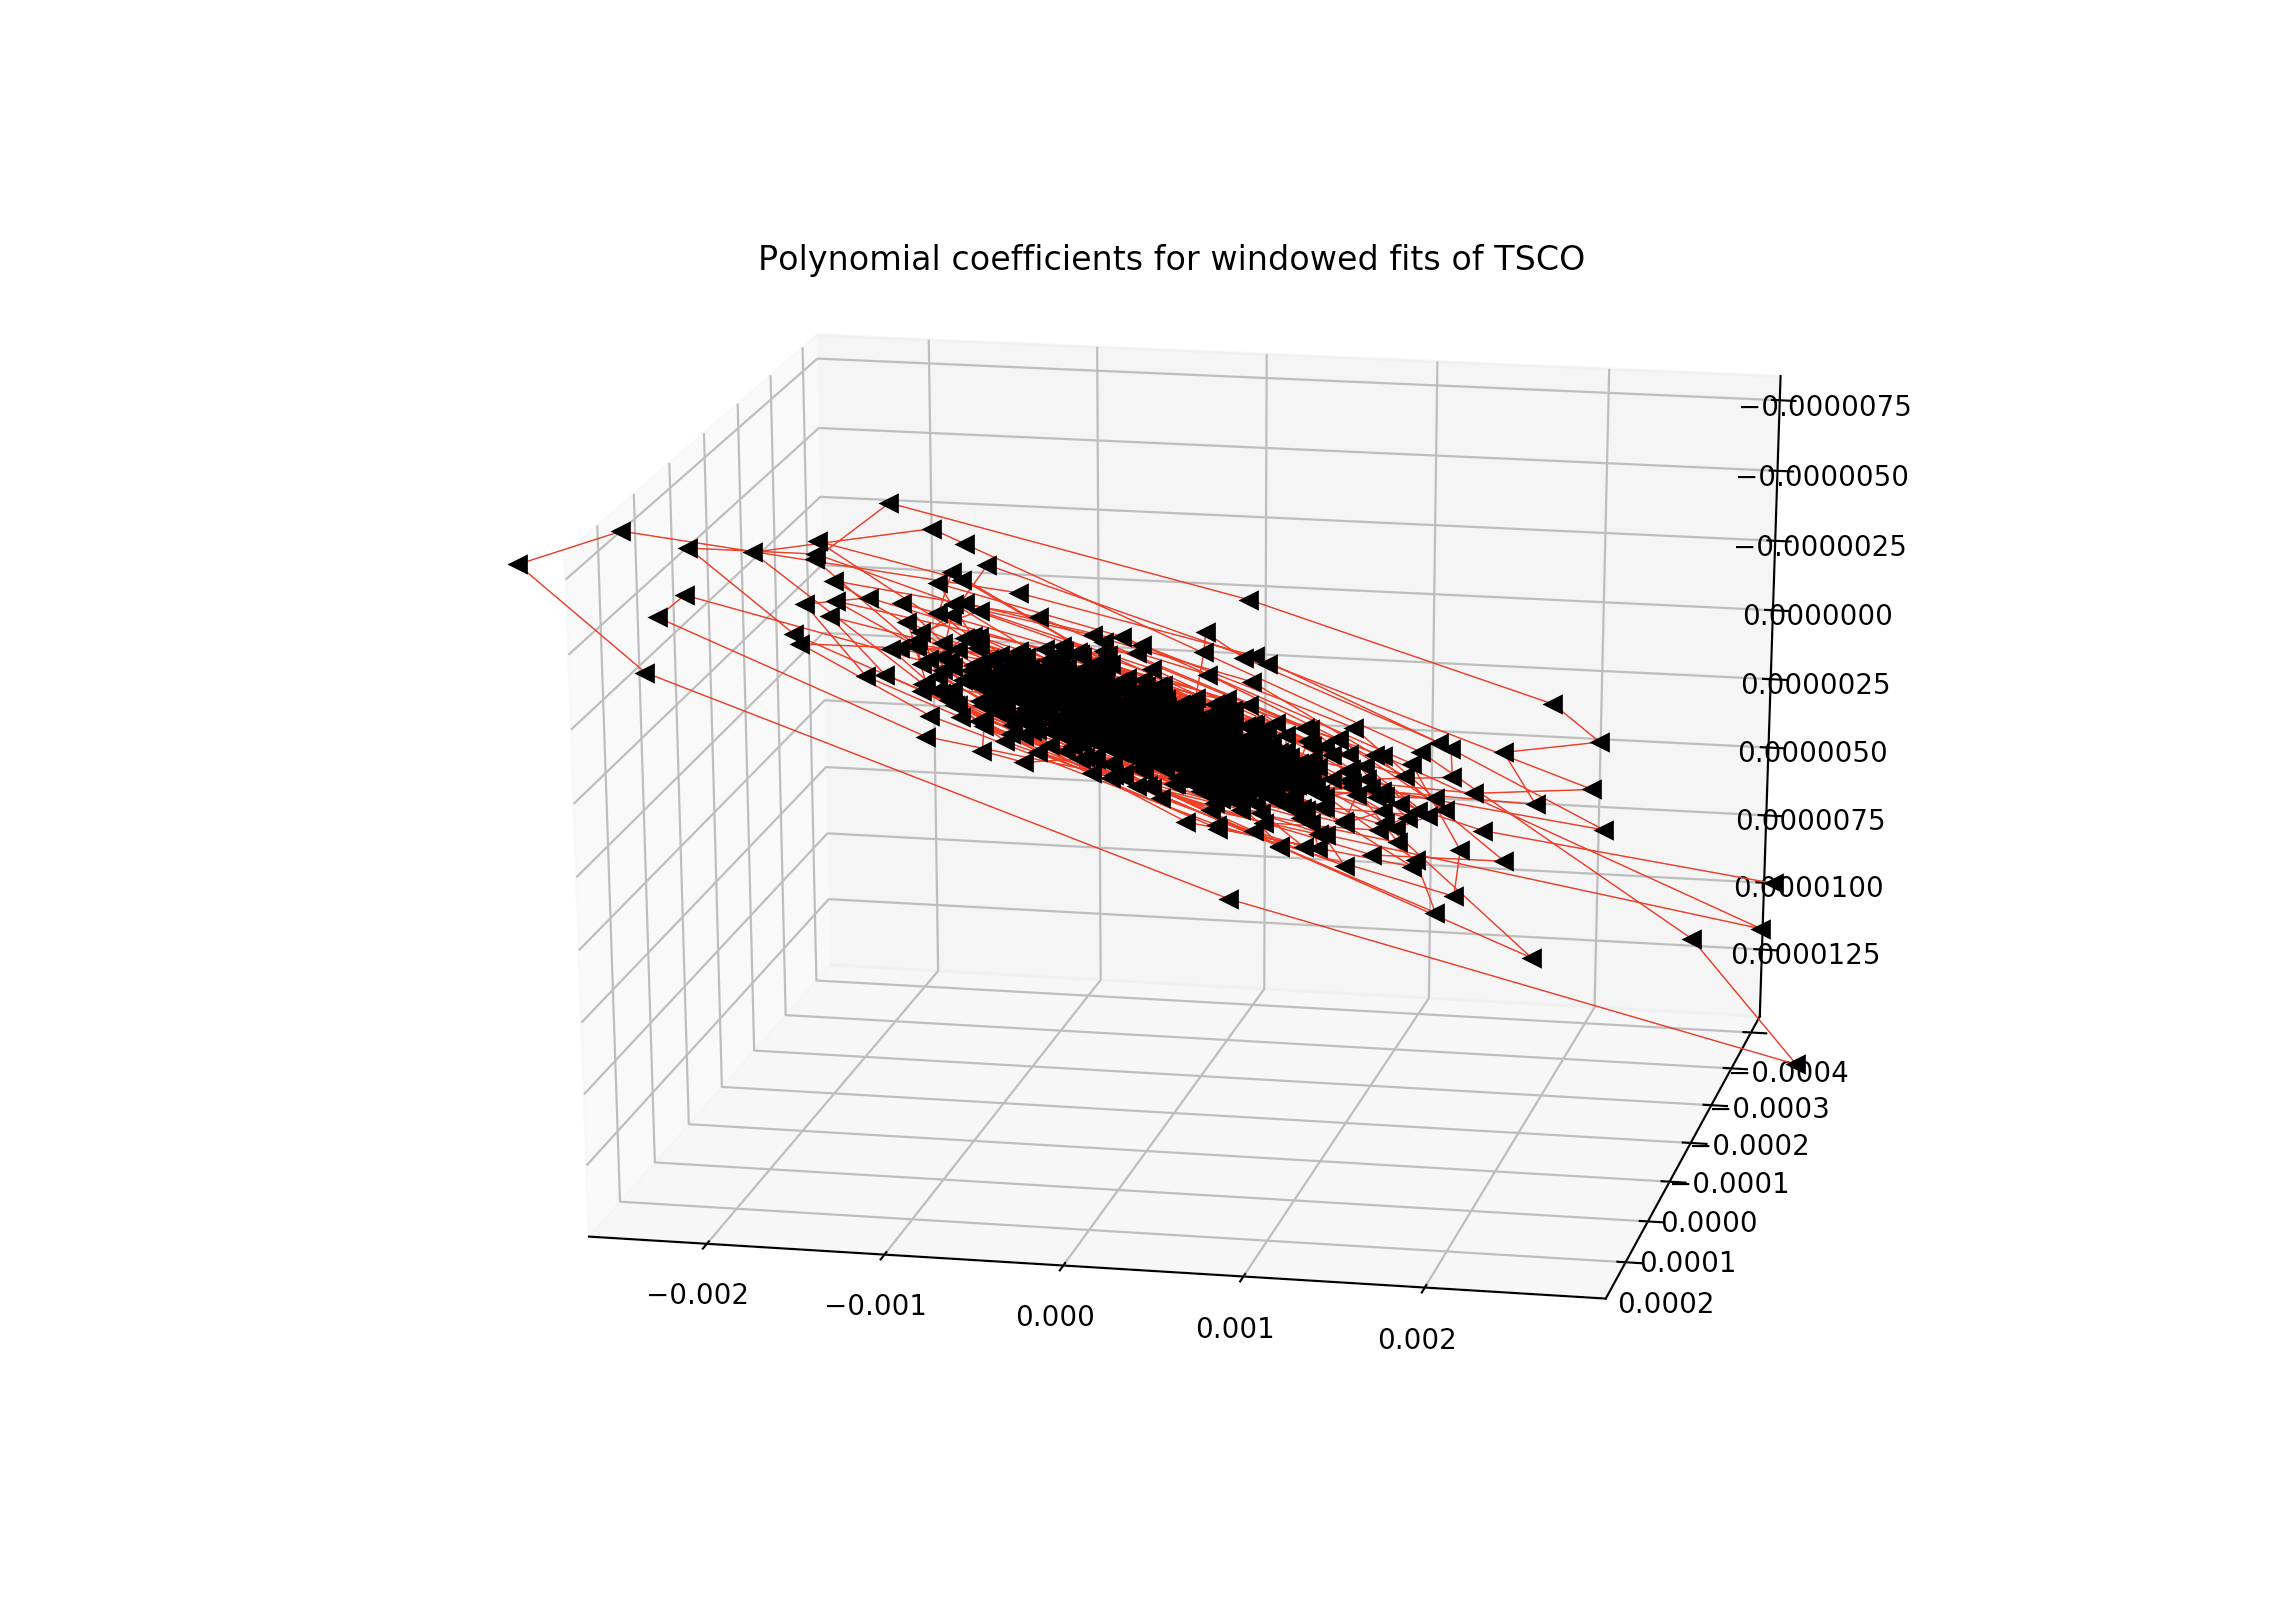
\includegraphics[width=\linewidth]{img/coeff1}
  \end{subfigure}
  \begin{subfigure}{.45\textwidth}
    \centering
    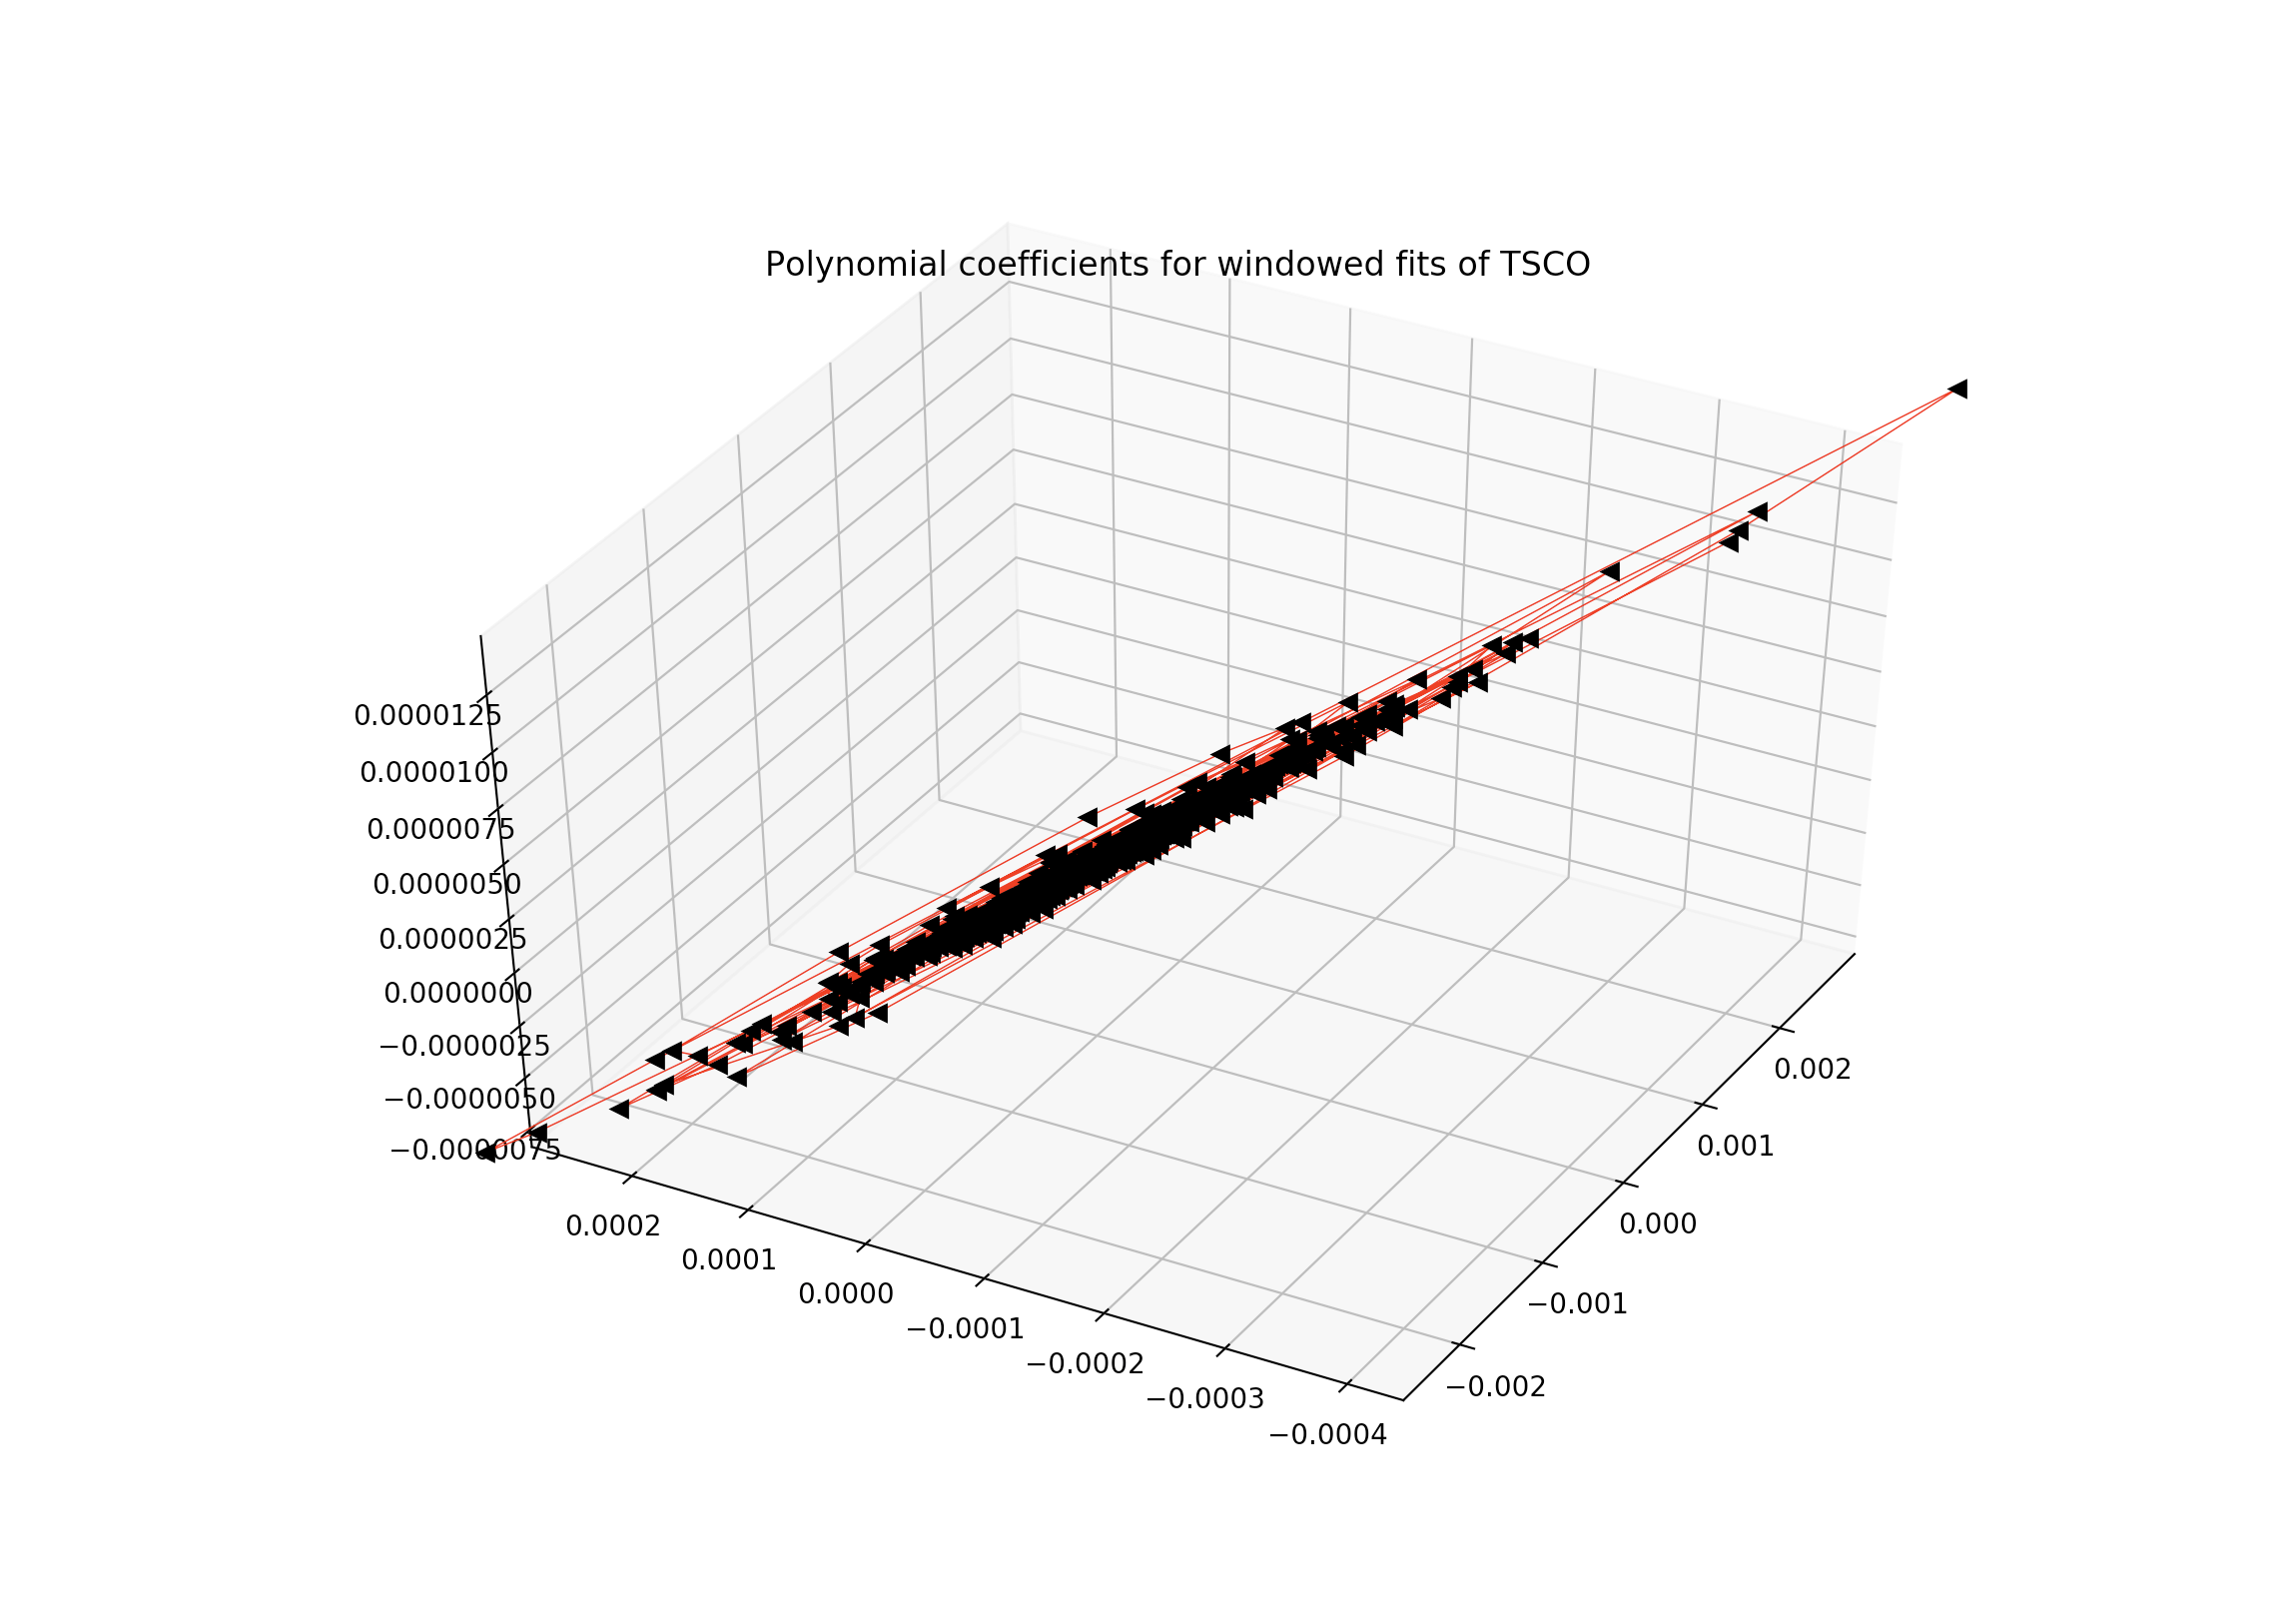
\includegraphics[width=\linewidth]{img/coeff2}
  \end{subfigure}
  \caption{Visualization of the lower order coefficients in $\mathbb{R}^3$}
  \label{fig:coeff12}
\end{figure}

The distribution of the coefficients in three dimensional space seems
to be a multivariate Gaussian distribution. Furthermore, it seems to
be very flat, appearing to be a line if viewed from the correct angle.

We experimented with different window sizes and different amounts of
shifting between consecutive windows. We found that in general,
varying the window sizes did not affect the shape of our graphs much
but the amounts of shifting affected the smoothness and trajectories
of our graphs. If the amount of shifting was large, such as if it were
half the size of a window, then the trajectory would be very rough and
edgy. If this value were to increase even more such that there was no
overlap between windows, the trajectory would be random, as shown
below.

\begin{figure}[H]
  \centering
  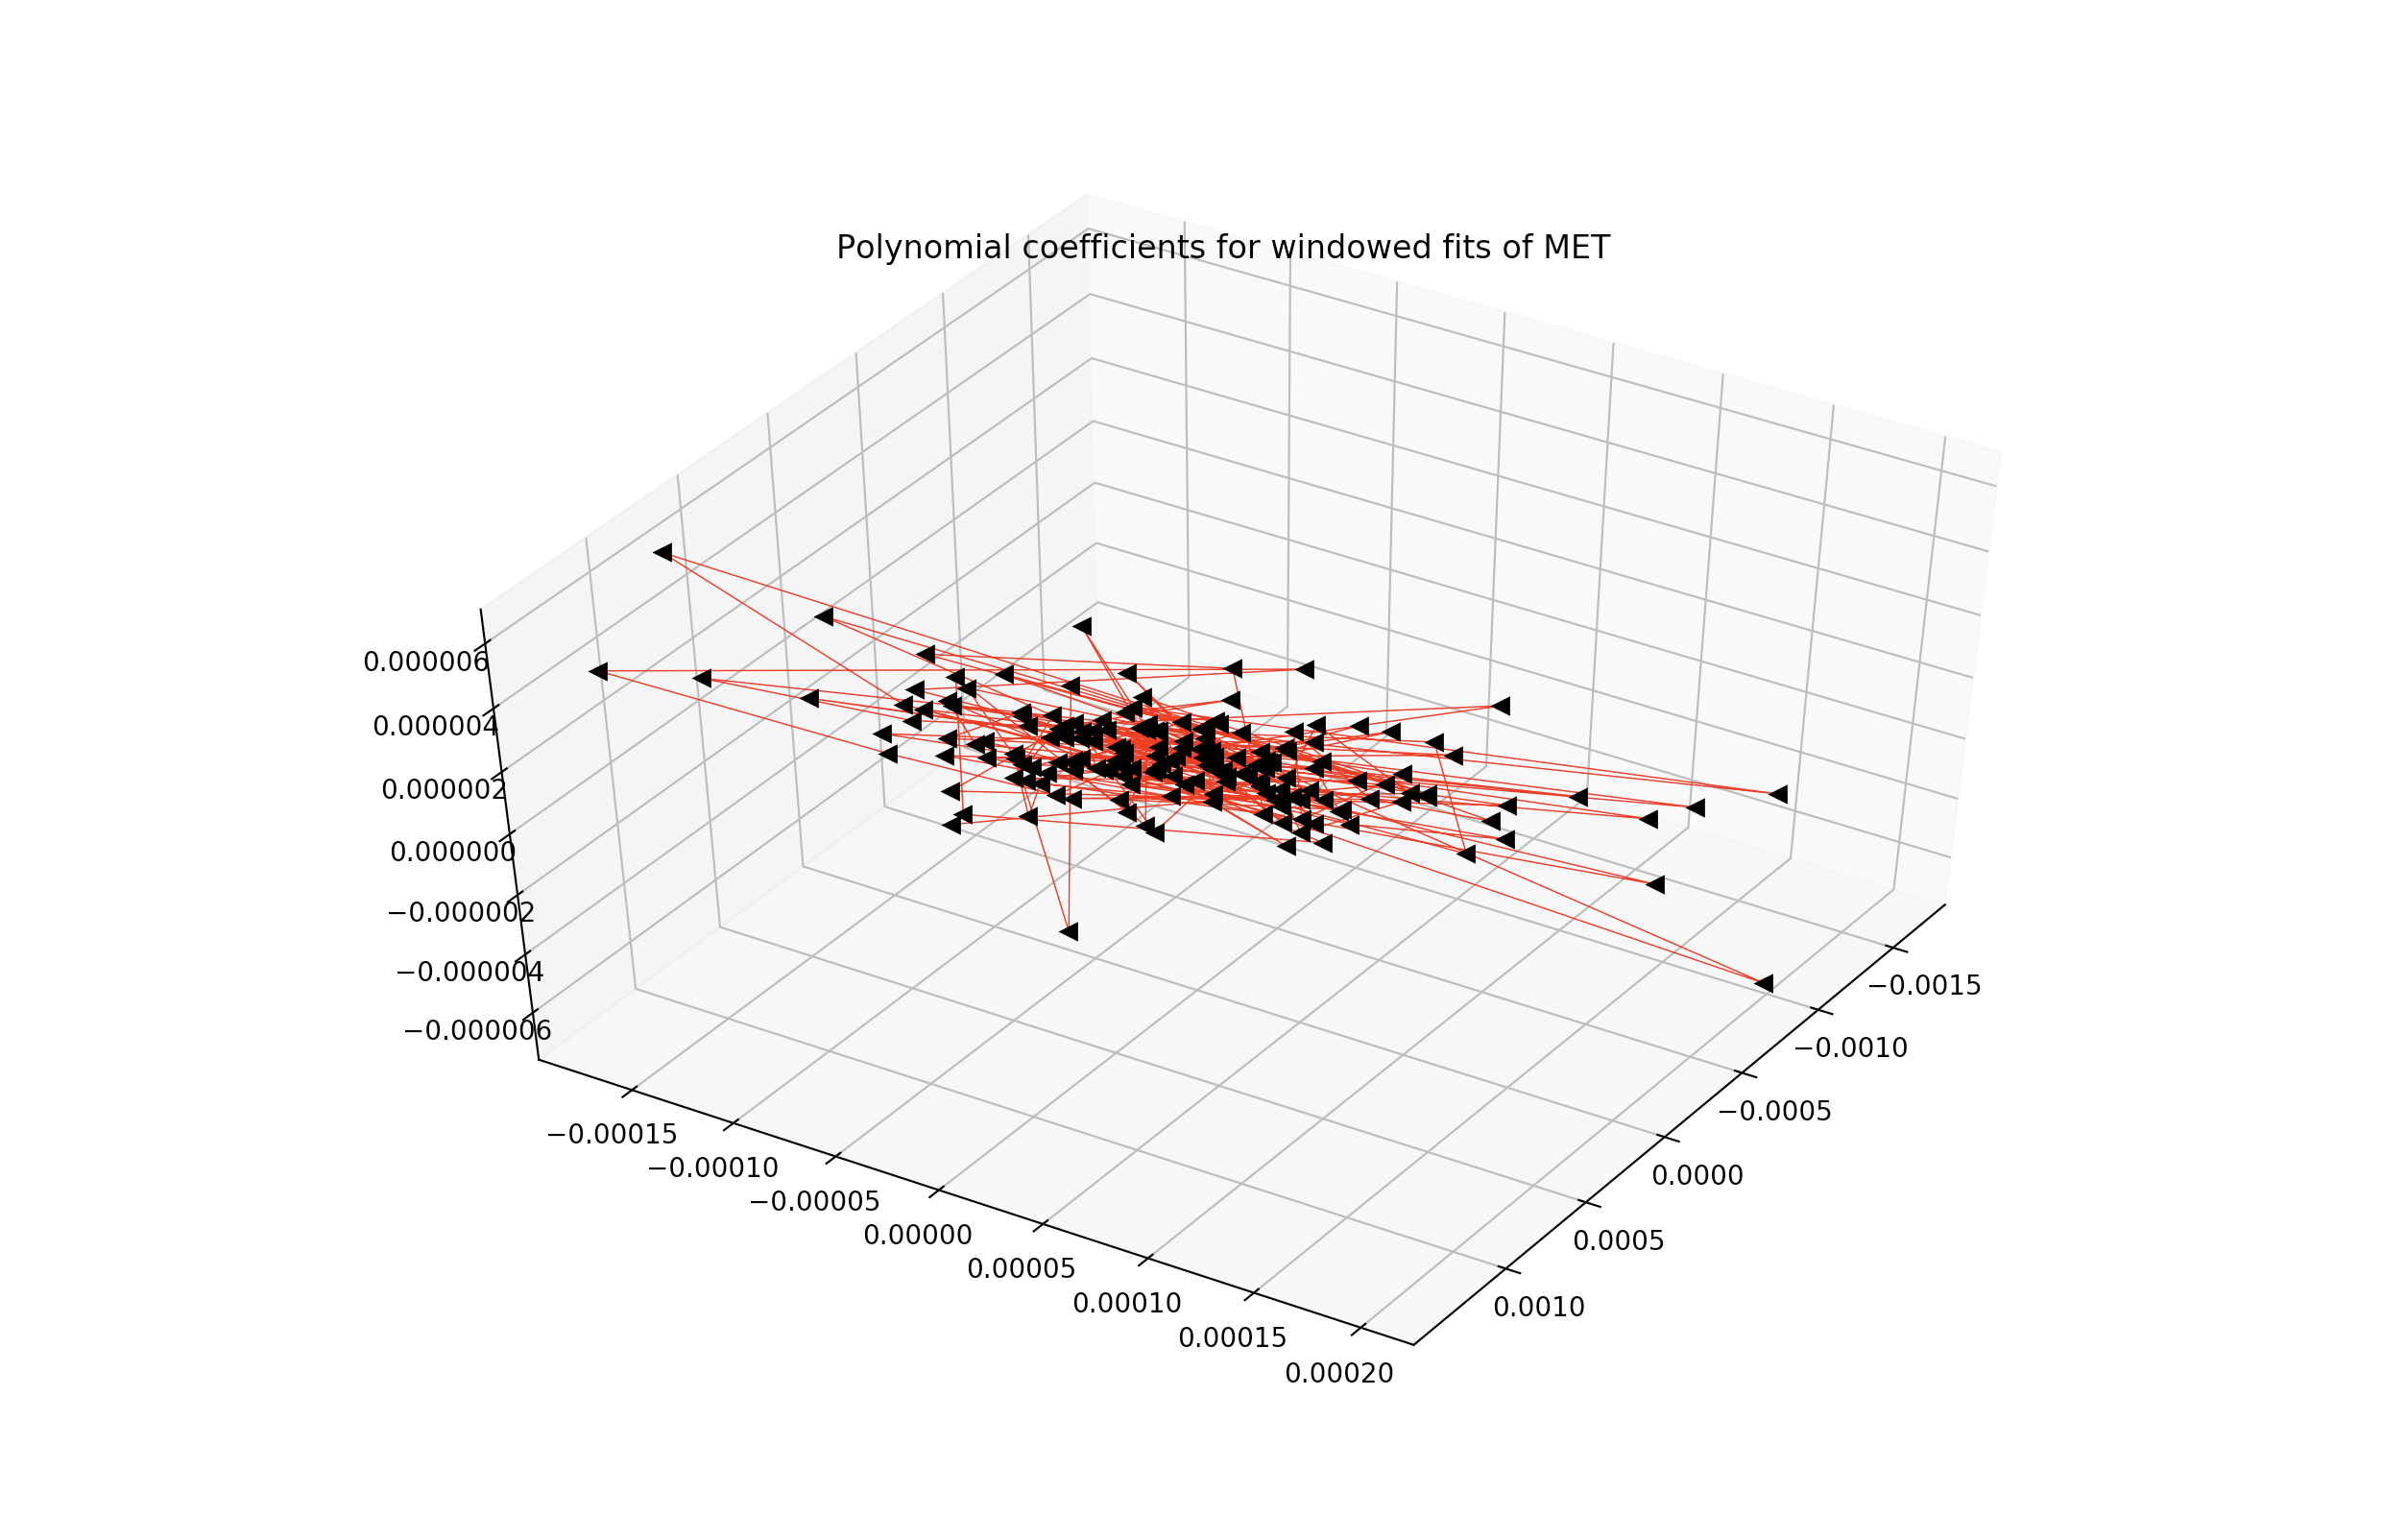
\includegraphics[width=\linewidth]{img/coeff3}
  \caption{Visualization of the lower order coefficients in $\mathbb{R}^3$
  without overlapping windows}
  \label{fig:coeff3}
\end{figure}

Although it is hard to see on the diagrams above, we noticed that the
trajectory of coefficients seemed to be rotating about the center of
the distribution. Thus, we wanted to examine the following questions
about this representation of the data:
\begin{enumerate}
  \item Why is the distribution so flat? Are the coefficients maybe
    not as independent from one another as we believed?
  \item Why might we be seeing this periodic behavior? And can we use
    Fourier analysis to extract meaningful information about it?
\end{enumerate}
For the first, we have a few theories: first, for a degree $N$
polynomial, the coefficients are really only controlled by $N-1$
variables: the roots. Hence, our solutions might be constrained to
some hyperplane. Second, it could be that regularization is
constraining the coefficients to the plane, preventing any one term
from getting too large. So, satisfied with this answer for the time
being, we moved on to Fourier analysis.

\subsubsection{Discrete Fourier Transform}

We would like to be able to compare stocks and be able to say how
similar two stocks are based on trends. To do this, we need some
quantitative measure of the stock trends. The vectors of coefficients
that we have are insufficient for several reasons. For one, we could
have two stocks whose behavior is almost exactly the same except one
is a scaled and shifted version of the other. To remedy this
situation, we could do some sort of scaling of shifting of our
coefficients but that may be difficult and impractical since the two
stocks may in fact be different and this sort of scaling and shifting
would be computationally intensive and pointless. Another issue that
we may run across is that two stocks may resemble each other in two or
more different disjoint periods of time but differ elsewhere. This
resemblance is something we want to consider since this can help us in
predicting the future behavior of our stocks. If we attempt to perform
this scaling and shifting operation on the coefficients, we may at
best have one of these similar regions overlap. We could try scaling
and shifting subsets of our coefficients but that would be even more
computationally expensive. To remedy the situation, we have to find a
new metric by which we compare two different stocks and their trends.

We decided that analyzing the periodic behavior of our stocks would
capture this information better. We hypothesize that two similar
stocks will have similar periodic behavior. To extract information
about the periodicity of our data, we performed a discrete fast
Fourier transform on each of our coefficient vectors, i.e. we
performed the Fourier transform on all the constant terms in each
window to extract information about the periodicity of the constant
terms, then another transform on all the linear terms, etc. We decided
to perform the Fourier transform on the coefficients instead of the
actual stock prices because we wanted to see if this abstraction would
yield any improvements in classification.

% TODO: fix the captions

\begin{figure}[H]
  \centering
  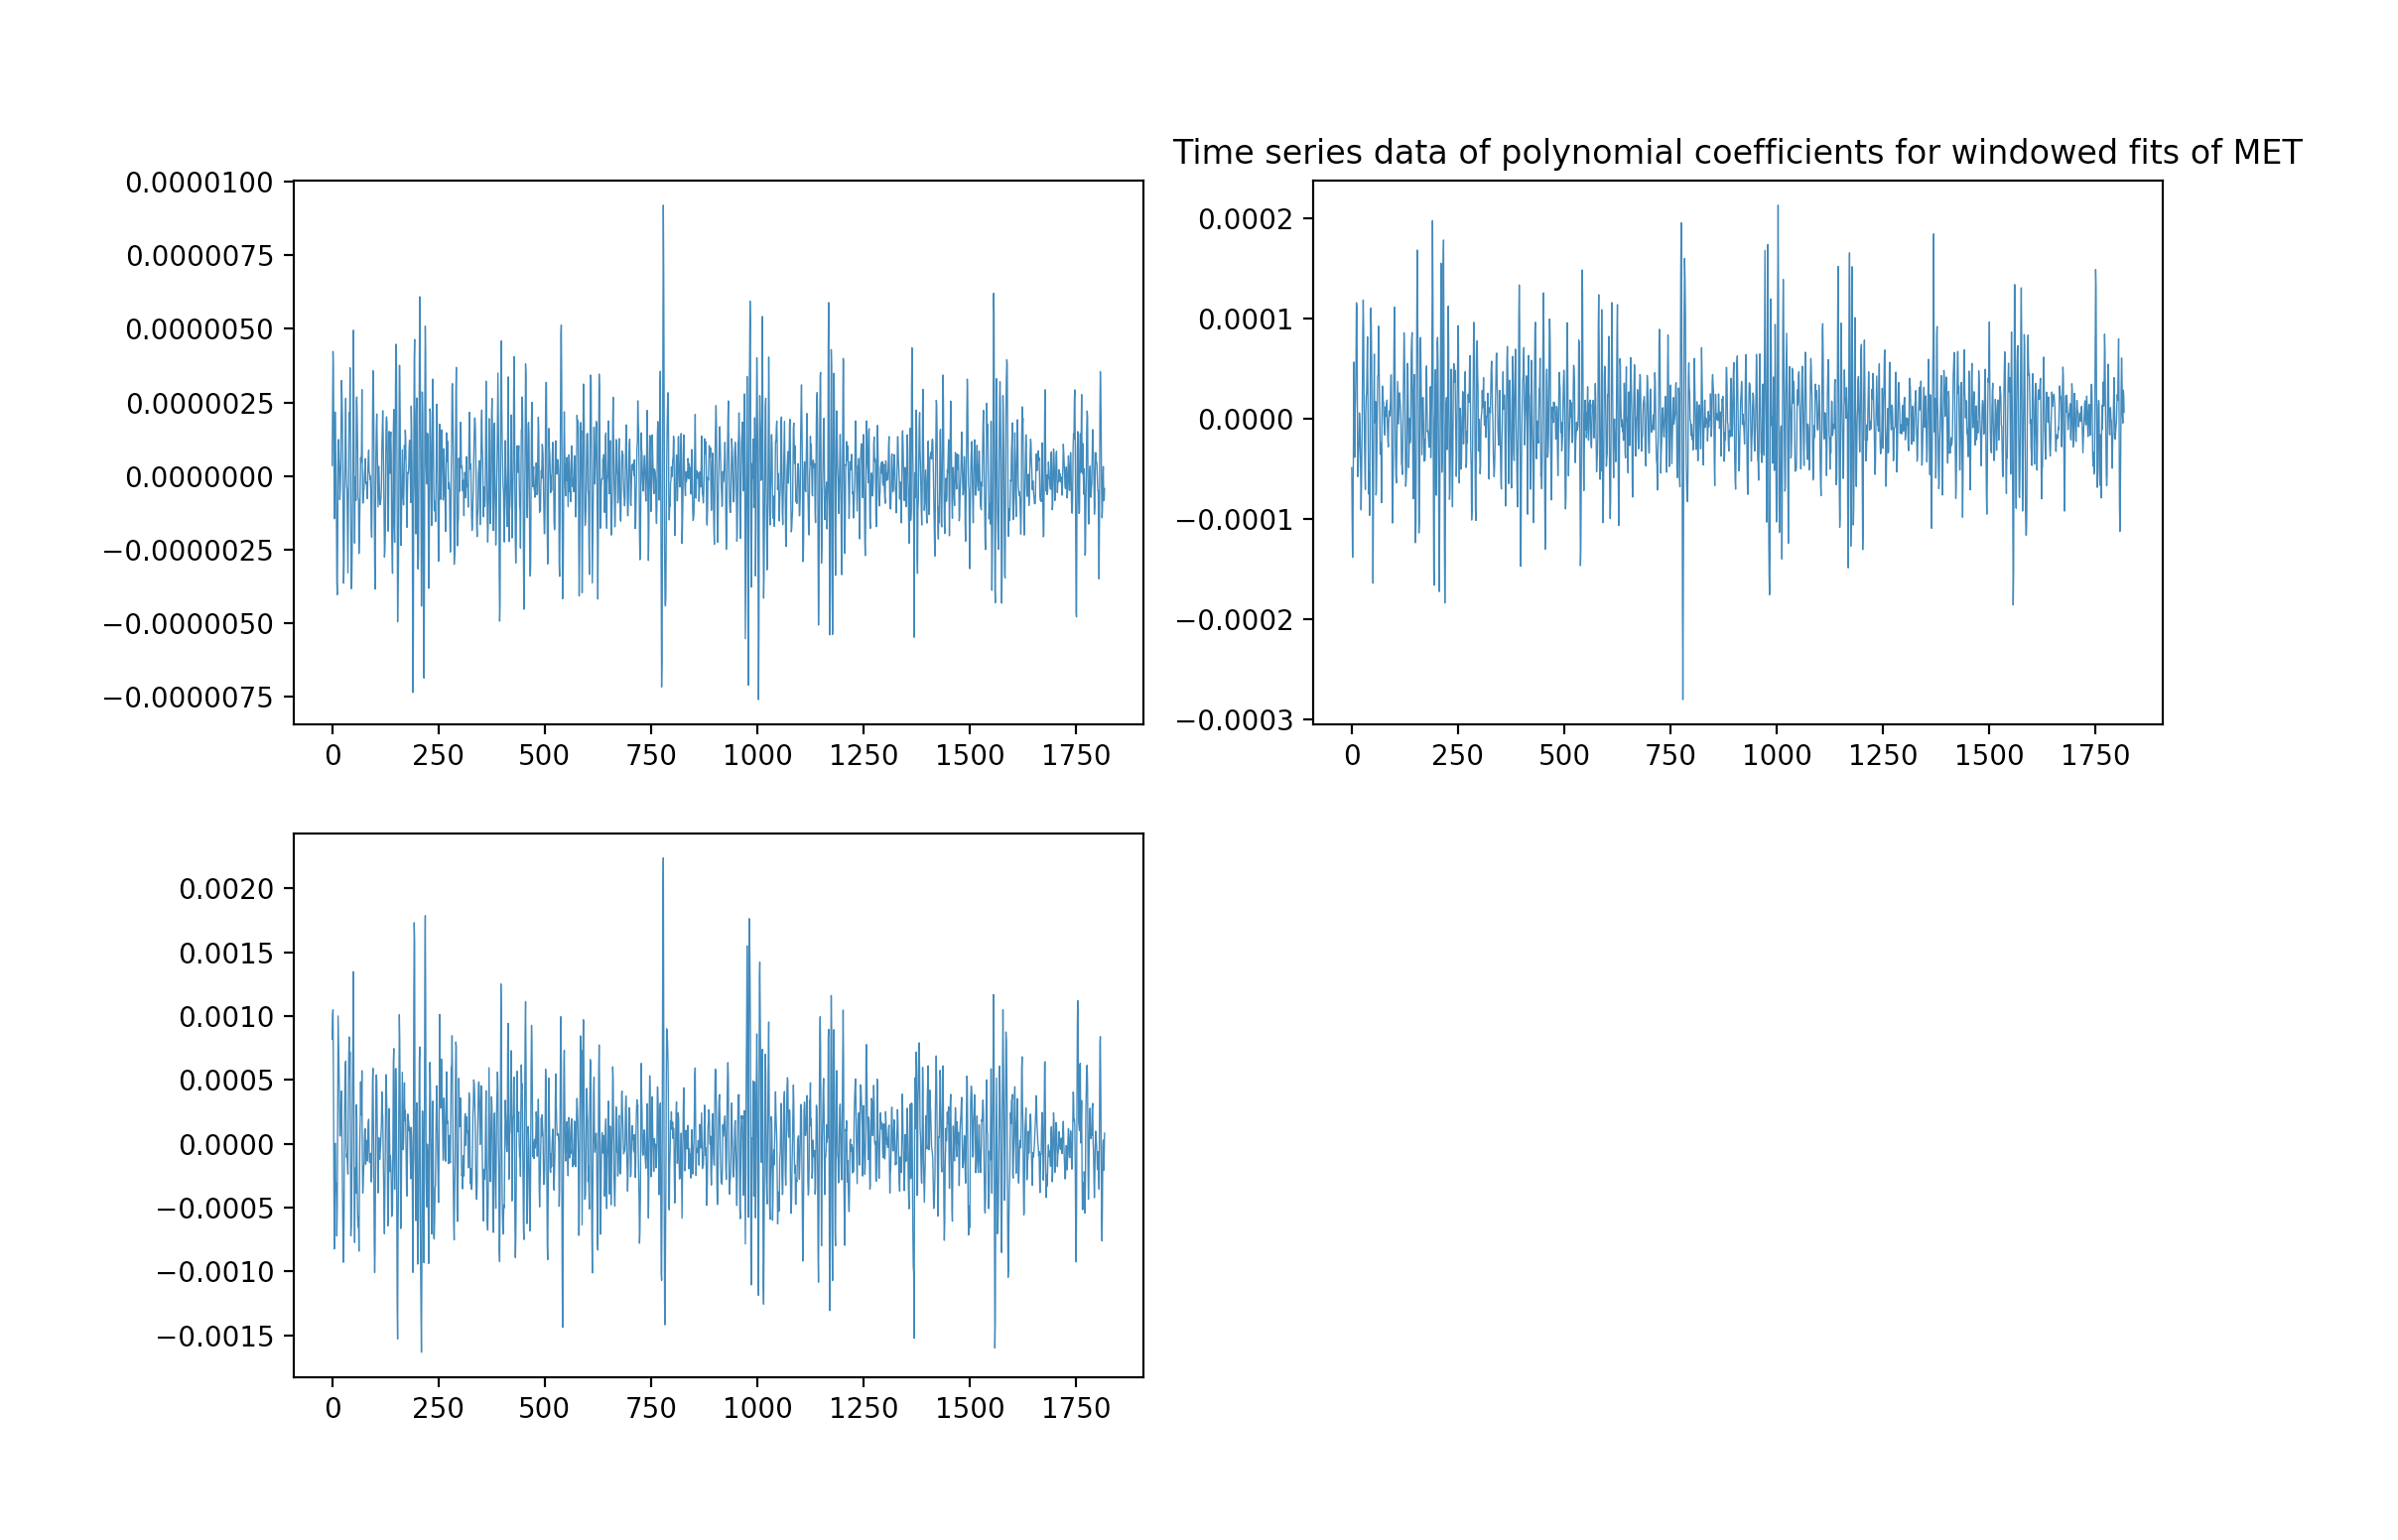
\includegraphics[width=.55\linewidth]{img/fourier1}
  \caption{Visualization of the lower order coefficients in $\mathbb{R}^3$
  without overlapping windows}
  \label{fig:fourier1}
\end{figure}

\begin{figure}[H]
  \centering
  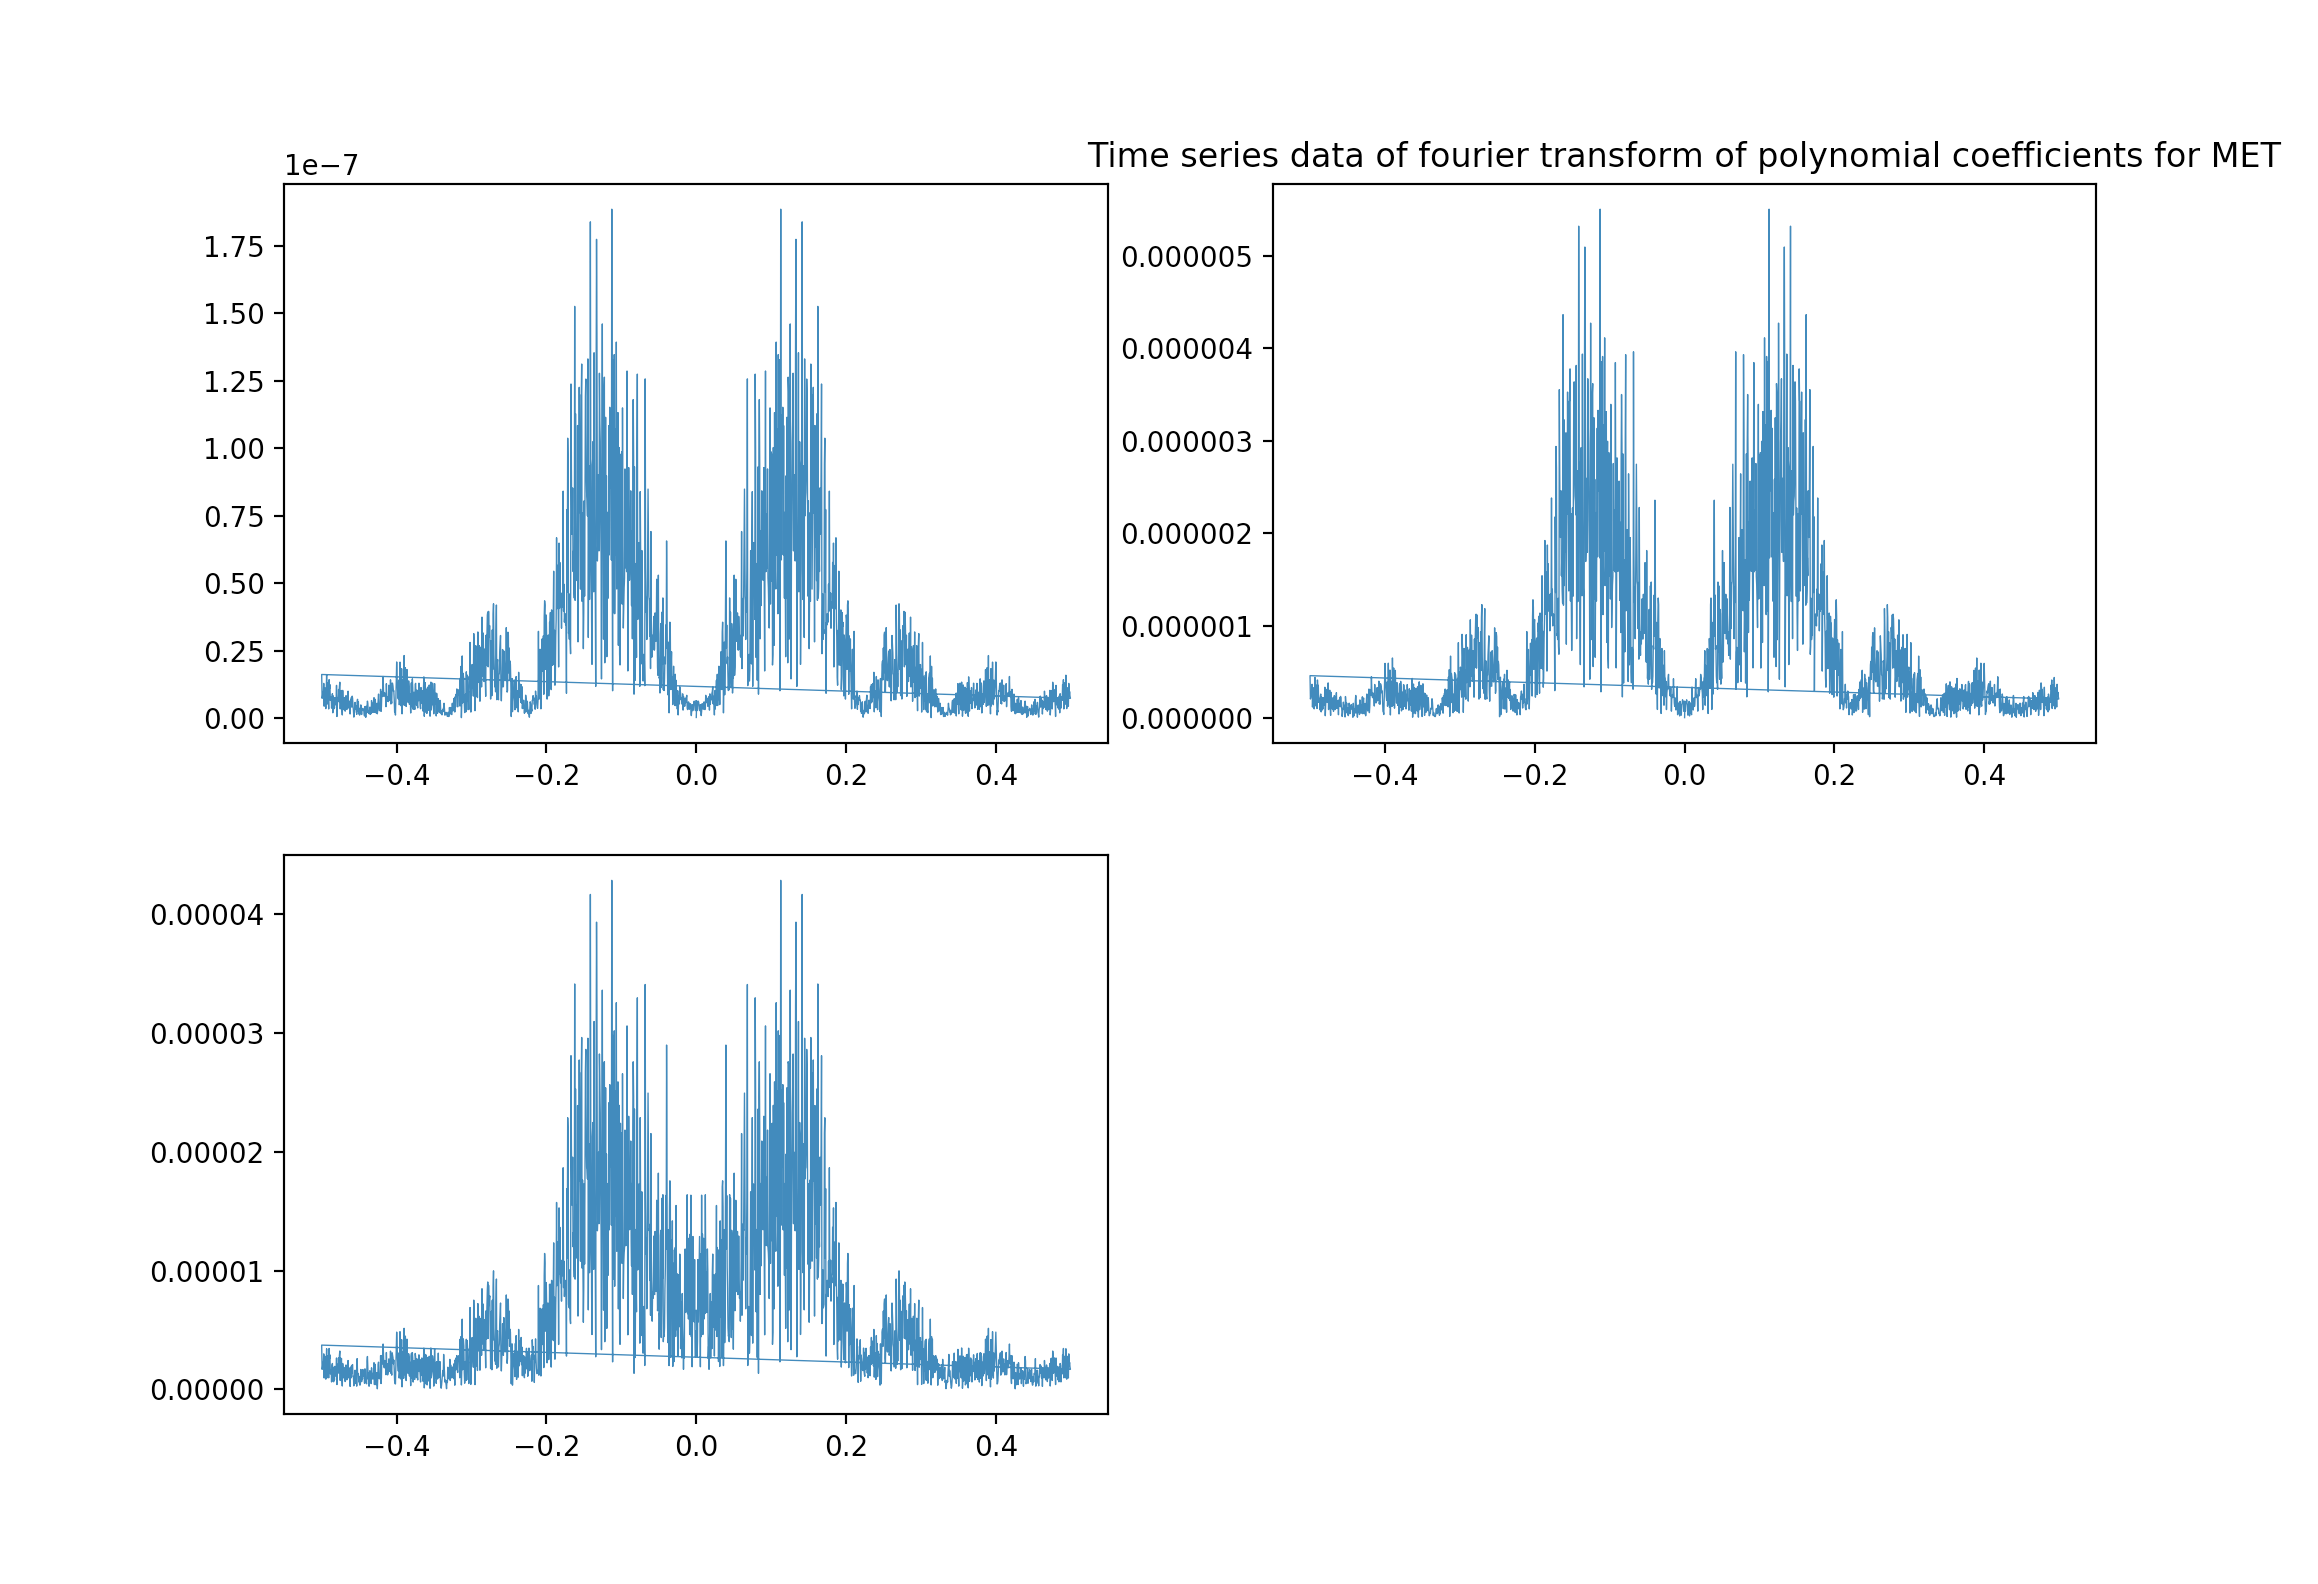
\includegraphics[width=.55\linewidth]{img/fourier2}
  \caption{Visualization of the lower order coefficients in $\mathbb{R}^3$
  without overlapping windows}
  \label{fig:fourier2}
\end{figure}

\begin{figure}[H]
  \centering
  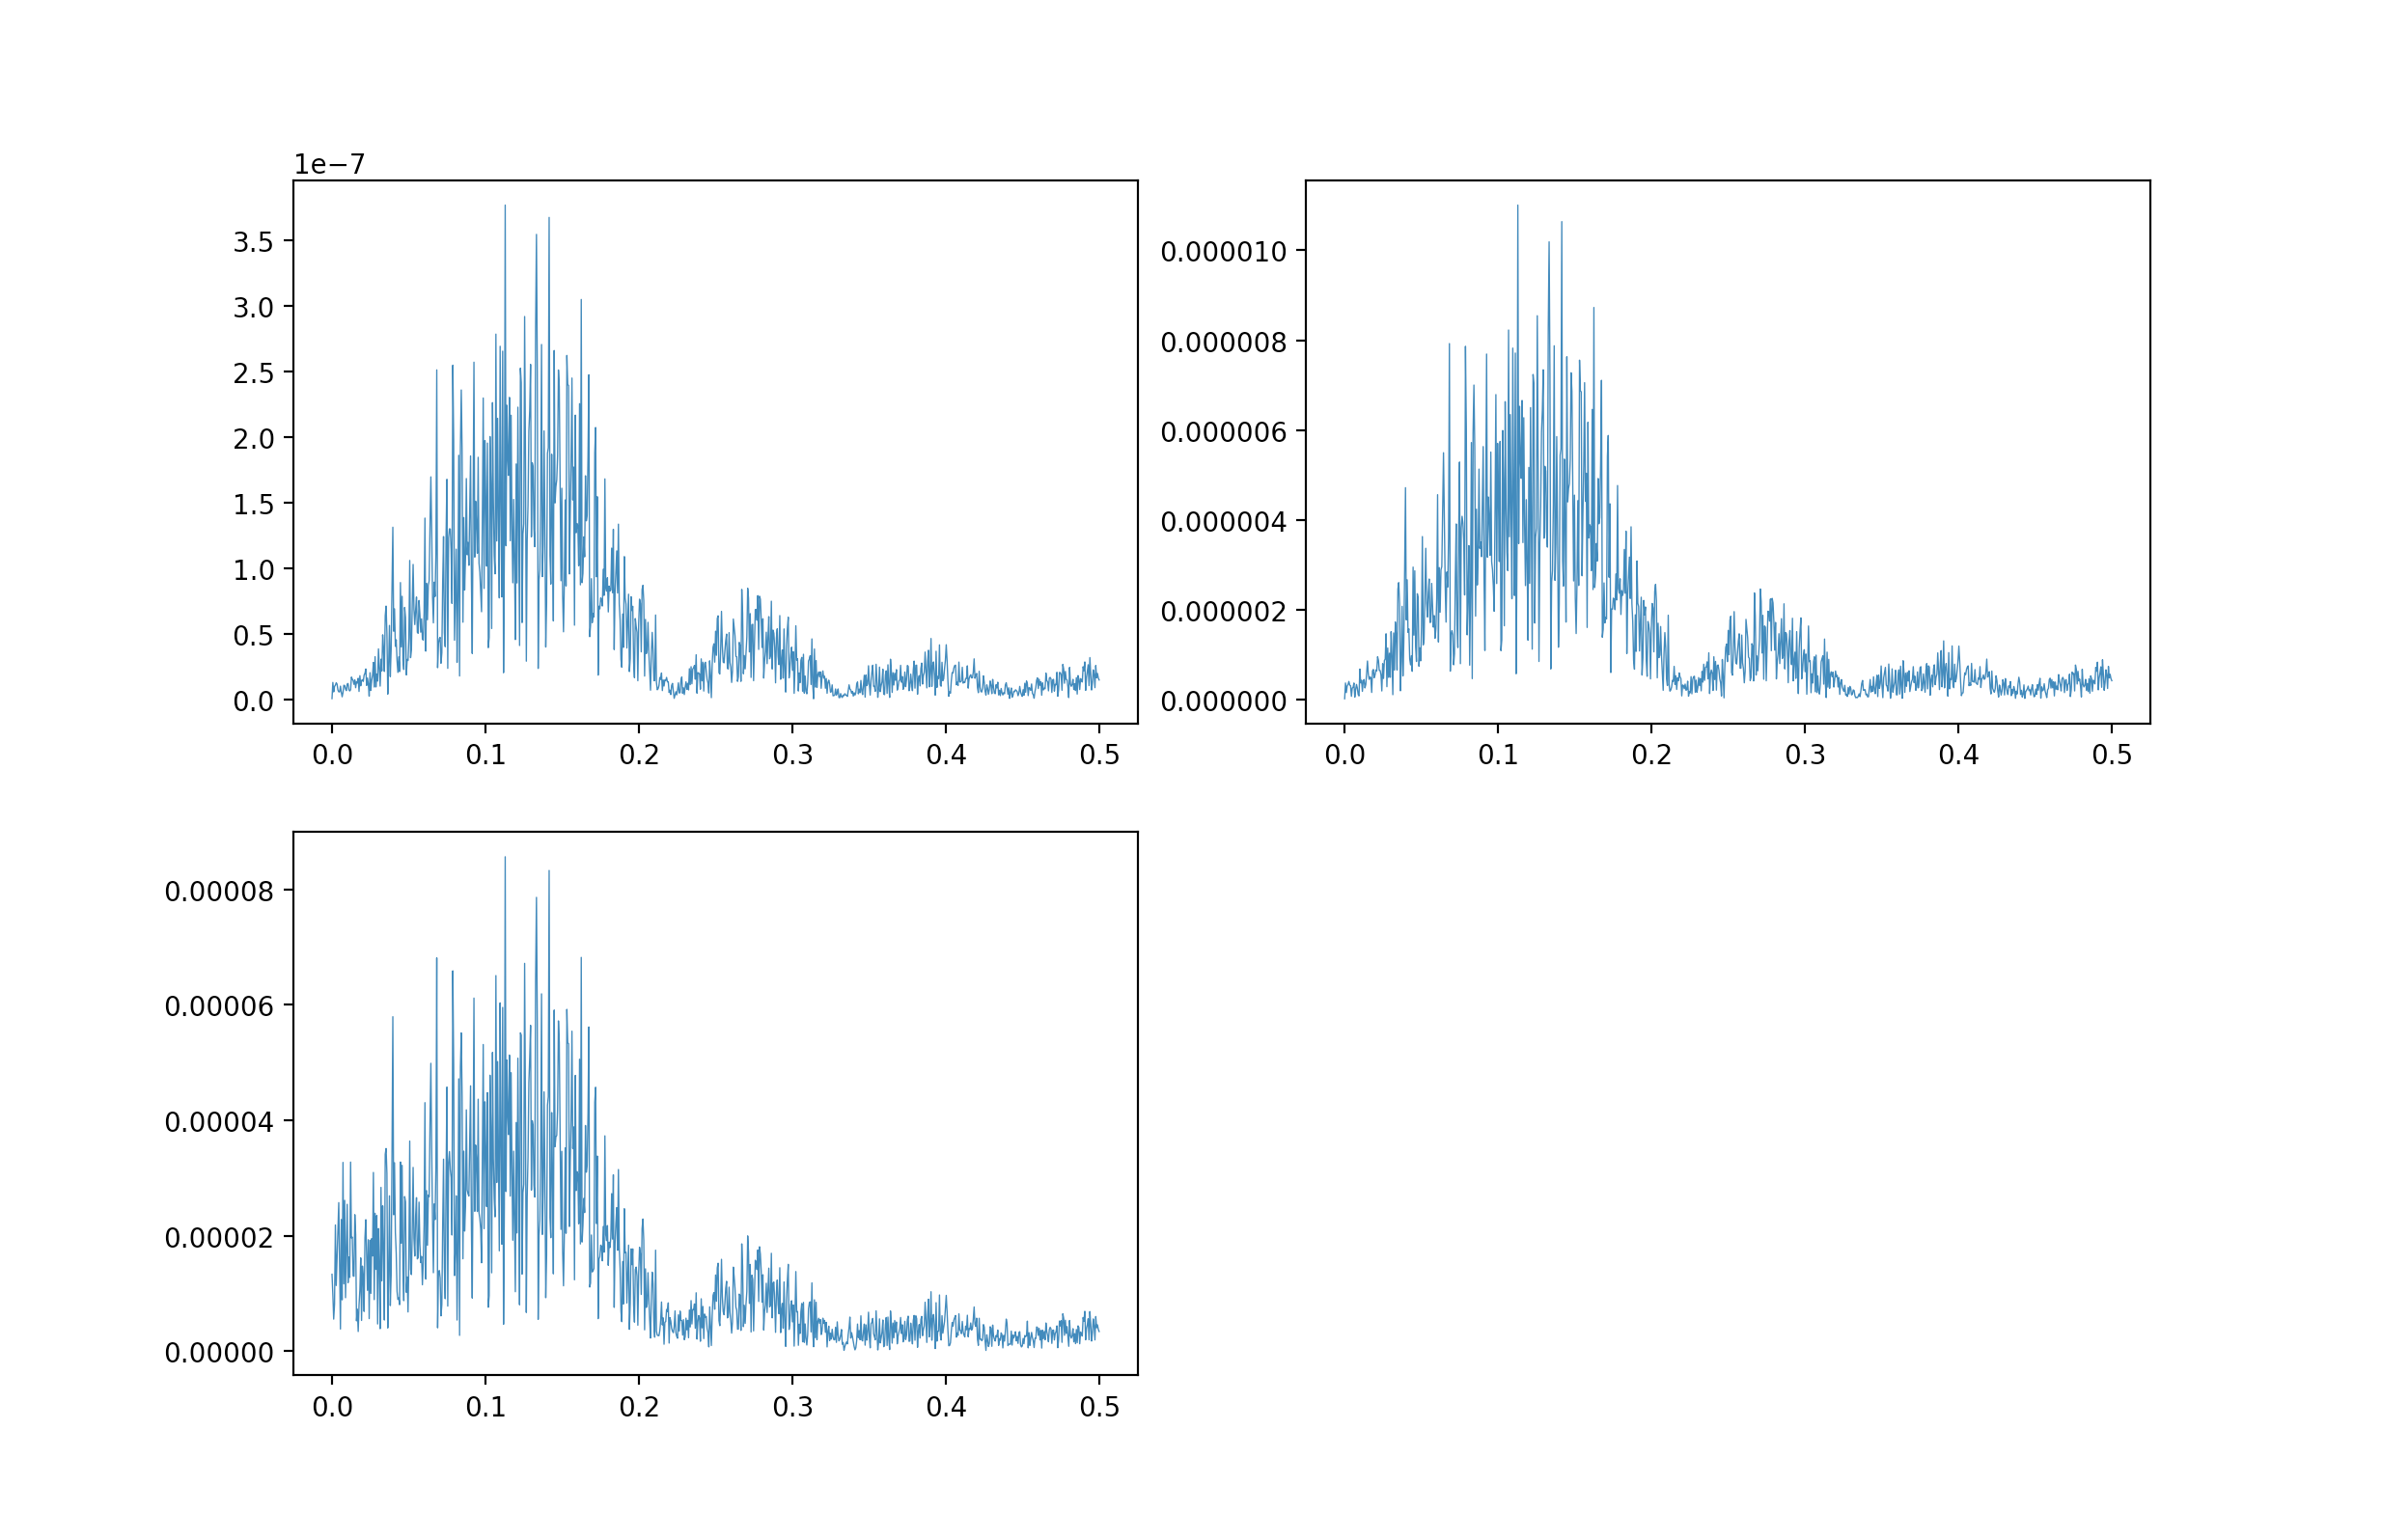
\includegraphics[width=.55\linewidth]{img/fourier3}
  \caption{Visualization of the lower order coefficients in $\mathbb{R}^3$
  without overlapping windows}
  \label{fig:fourier3}
\end{figure}

\subsubsection{K-means Clustering}

In this section, we'll give an overview of the techniques that we
applied to get results for the final presentation, then move into the
optimizations and corrections that we applied in the following days.

We decided to apply a K-means algorithm to our fourier coefficients,
to try and get some clustering behavior. Because each stock was fitted
with a quintic polynomial, our fourier data for each stock looked
something like
\begin{align*}
  \mathcal{F}(\texttt{GOOGL})
  &=
    \begin{bmatrix}
      a_{0,0} & a_{0,1} & \cdots & a_{0,n} \\
      a_{1,0} & a_{1,1} & \cdots & a_{1,n} \\
      \vdots & \vdots & \ddots & \vdots \\
      a_{6,0} & a_{6,1} & \cdots & a_{6,n}
    \end{bmatrix}
\end{align*}
where $a_{i,j}$ is the complex amplitude for the $j^{\text{th}}$
frequency in the discrete fourier transform of the coefficient for the
term of degree $i$. Here, $n$ represents the number of total
frequencies in our DFT, as documented in \texttt{np.fft.fftfreq}.

Since we were analyzing a total of 299 stocks, we really have a large,
$299 \times 6 \times n$ array of transformed data. Since our
\texttt{k\_means} function we wrote for homework takes data matrices
as input, we initially thought that we could just flatten each of the
$6 \times n $ fourier sub-arrays, and feed them into the
\texttt{k\_means} classifier. However, when we attempted to do so, we
saw significant performance dropoffs in the initialization of the
clusters. This was confusing, since we were able to initialize
clusters for individual coefficients' fourier vectors quite rapidly,
and the flattened versions were of the same order of magnitude (only 6
times larger). We suspect that either \texttt{np.ndarray.std()} or
\texttt{np.random.multivariate\_normal()} simply doesn't scale well if
one of the axes gets particularly elongated, but we'll look into it
further.

Anyways, for each, stock, we applied \texttt{np.abs()} to the fourier
matrix, so that we wouldn't have to rewrite \texttt{k\_means} to deal
with complex vectors. This is something we'd like to improve in the
future. Then, we applied \texttt{k\_means} clustering along each of
the rows. That is, for each stock, we did \texttt{k\_means} clustering
for the frequency vectors for each of the coefficients, iterating over
40 different values of $k$ to find an optimal number of clusters.

Then, for each stock, we applied a one-hot encoding to store
information about which cluster each of its coefficients were from.
After flattening this collection of one-hot vectors into a single
vector, we once again applied \texttt{k\_means} (iterating through 500
different values of $k$), and output the results.

One might wonder why we chose to use $500$ different $k$-values, as
we had only $299$ stocks. The reasoning was this: we knew our data lay
in a low-dimensional hyperplane of the original space, but the starter
code for \texttt{k\_means} initialized the clusters following a simple
multivariate gaussian distribution. Hence, many of the the centroids
would be far away from the data's hyperplane, and so for small $k$, we
were seeing stocks classified in just one or two clusters. We figured
that if we upped the number of clusters, we'd have a higher chance of
some of the randomly-initialized centroids being closer to different
regions of the data.

Admittedly, this algorithm is quite crude, but as a minimum viable
product, we weren't too concerned with performance issues, and are
willing to revisit accuracy concerns in the future.

\subsection{Markov Chain Prediction}

\subsubsection{Slope Estimation}

For each sliding window, the difference in height between the last point and
the first point was taken as an approximation for the slope of the trend of
that window. We were interested in the slope because it is an indicator for
whether the stock price is falling, stable, or rising.

\subsubsection{Data Binning}

We then decided to bin our data since the slopes were real numbers and binning
the data was necessary to be able to use a Markov model. Otherwise, it would be
extremely likely that our model would not have seen the slope data of the stock
that we were predicting.

We binned our slopes according to the following scheme.

% TODO: fix spacing

\begin{verbatim}
7.5  < x         ->   3
4.5  < x <  7.5  ->   2
1.5  < x <  4.5  ->   1
-1.5 < x <  1.5  ->   0
-4.5 < x < -1.5  ->  -1
-7.5 < x < -4.5  ->  -2
       x < -7.5  ->  -3
\end{verbatim}

The following graphs show the results of the slope extraction and data binning
for four of our stocks.

\begin{figure}[H]
  \centering
  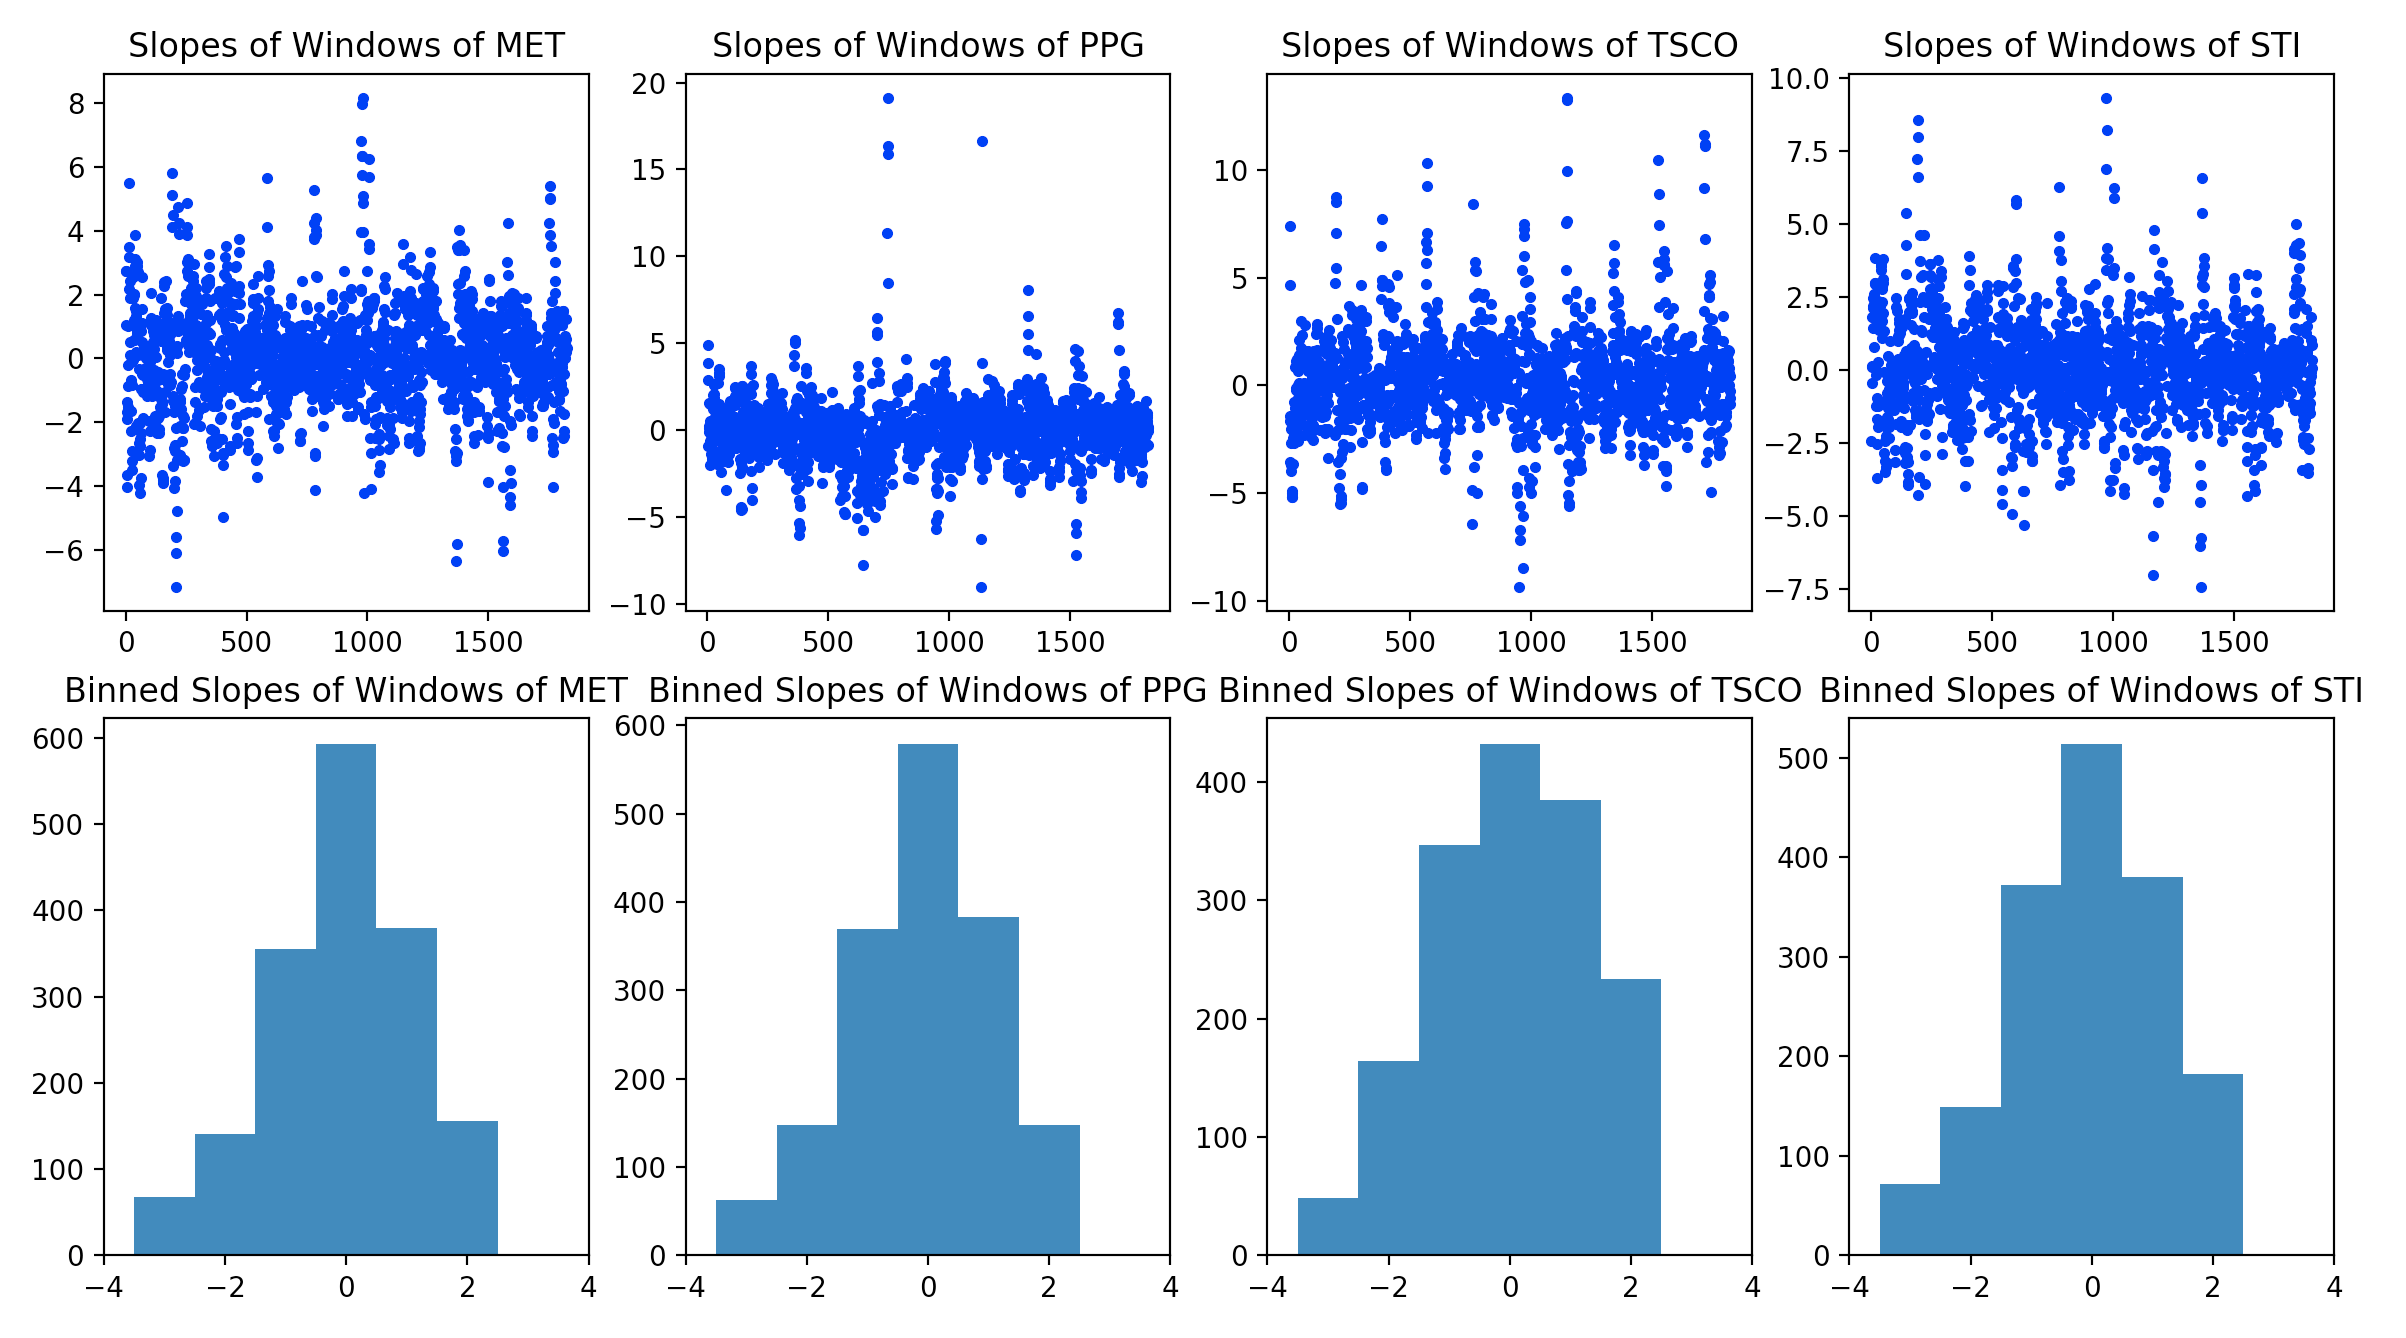
\includegraphics[width=\linewidth]{img/slopes}
  \caption{Graphs of slopes and binned slopes for four different stocks}
  \label{fig:slopes}
\end{figure}

\subsubsection{Markov Model}

We then fed all the slope data into a Markov model. Given any two consecutive
binned slopes, our model would provide a list of all the succeeding binned
slopes it had encountered in the training data immediately after seeing the two
provided consecutive binned slopes.

\subsubsection{Prediction}

Given the binned slopes of the two most recent sliding windows for a stock, our
Markov model would be able to provide a vector of suggested choices in the form

\[
  \mathbf{y} = \Bigl<P_{sell}(\mathbf{x}), P_{nothing}(\mathbf{x}),
  P_{buy}(\mathbf{x})\Bigr>
\]

It does this by taking the list of upcoming slopes from the Markov model and
collapsing them into counts by putting the binned slopes into three different
bins according to the following scheme.

\begin{verbatim}
-3    ->  sell
-2    ->  sell
-1    ->  do nothing
 0    ->  do nothing
 1    ->  do nothing
 2    ->  buy
 3    ->  buy
\end{verbatim}

The counts are then normalized to make it a probability distribution.

\section{Results}

\subsection{K-means}

\subsubsection{Performance}

Although quite unoptimized, our algorithm completed analysis of $\sim
2,100,000$ data points in just $\sim 4$ minutes. The process of
windowed fitting for all 299 stocks took roughly $40.6$ seconds, while
the two iterations of \texttt{k\_means} took about $223.1$ seconds on
my macbook (including the hyperparameter search for optimal $k$, which
comprised the bulk of the computation time).

This is very promising, as it indicates that our algorithm would
perform fast enough to be used in real-time, given a decently-powerful
server. First, note that we'd only need to apply fitting to one window
at a time as new data is imported, which would take fractions of a
second. Second, note that the DFT has excellent performance for the
typical array lengths we're feeding it. Third, note that if we were
applying this sort of algorithm in real-time, we wouldn't expect the
optimal values of $k$ to change much between runs (especially if we
find a cleverer way to initialize centroids). Hence, we'd only have to
scan over a few values of $k$, a process that could be parallelized
extremely easily. Thus, we'd be able to perform a full run of our
algorithm in just a few seconds. Since the alphavantage API updates
every minute, this is more than fast enough to process the incoming
data.

\subsubsection{Output clusters}

Here is a partial list of some of the output clusters for one run of
the data:

\begin{table}[H]
\centering
\caption{Cluster 1}
\label{c1}
\begin{tabular}{@{}cl@{}}
\toprule
Count & Industry  \\ \midrule
1 & Cybersecurity \\
\bottomrule
\end{tabular}
\end{table}

\begin{table}[H]
\centering
\caption{Cluster 2}
\label{c2}
\begin{tabular}{@{}cl@{}}
  \toprule
  Count & Industry  \\ \midrule
  7 & pharmaceutical + biotech research \\
  3 & healthcare providers \\
  1 & health insurance \\
  1 & chemical supplier \\
  1 & scientific research \\
        & \\
  2 & construction / motor supplies \\
  1 & automobile company \\
        & \\
  1 & natural gas / petroleum \\
  1 & energy holdings \\
  1 & energy engineering / analysis firm \\
        & \\
  3 & airline \\
  1 & travel booking company \\
  1 & travel software company \\
        & \\
  1 & shipping company \\
        & \\
  3 & public utility providers \\
        & \\
  4 & financial firms \\
  2 & real estate investment firms \\
        & \\
  2 & food companies \\
  1 & grocery store real estate firm \\
  1 & mall real estate firm \\
  1 & office building / street real estate firm \\
  1 & casino \\
        & \\
  1 & media / news company \\
        & \\
  1 & telecom company \\
        & \\
  1 & storage company \\
  1 & xerox \\
        & \\
  1 & semiconductor manufacturer\\
  \bottomrule
\end{tabular}
\end{table}

\begin{table}[H]
\centering
\caption{Cluster 3}
\label{c3}
  \toprule
  Count & Industry \\ \midrule
  5 & oil / petroleum companies \\
  1 & energy engineering firm \\
    & \\
  2 & automotive parts manufacturers \\
  1 & tire / rubber manufacturer \\
  1 & motorcycle company \\
    & \\
  1 & heavy machinery rental business \\
  1 & freight transportation company \\
  1 & cruise company \\
  1 & airline \\
  1 & travel booking company \\
    & \\
  2 & semiconductor manufacturers \\
  1 & electronics manufacturer \\
  1 & applied materials science firm \\
  1 & low-level computer systems firm \\
  1 & network infrastructure firm \\
  1 & data storage company \\
  1 & data analytics firm  \\
    & \\
  1 & home appliance manufacturer \\
  & \\
  1 & office / business supplier \\
  1 & clothes supplier \\
  1 & cosmetics company \\
  & \\
  1 & life insurance \\
  & \\
  1 & biotech firm \\
  1 & pharmaceutical firm \\
  3 & health care firms \\
  & \\
  1 & computer systems / hardware supplier for hospitals \\
  1 & computer systems for biotech analysis \\
  2 & medical device manufacturers \\
  1 & implant / joint replacement manufacturers \\
  & \\
  1 & medical cannabis company \\
  & \\
  2 & paper companies \\
  & \\
  1 & telecom company \\
  & \\
  2 & financial firms \\
  1 & mutual fund \\
    & \\
  1 & entertainment / media company \\
  \bottomrule
\end{tabular}
\end{table}

% 5:
%         2 household product manufacturer
%         1 glass / can manufacturers

%         1 bubble wrap / vacuum packing
%         1 adhesive / etc. manufacturer

%         1 home improvement retailer
%         1 department store
%         1 walmart

%         1 fashion

%         1 management consulting service
%         1 investment management company
%         1 investment consulting + risk assessment
%         1 risk management consutling

%         2 video game company
%         1 productivity software (adobe)

%         1 google
%         1 amazon
%         1 HP (hewlett-packard)
%         6 broadcast / network infrastructure
%         2 content delivery / cloud computing
%         2 integrated circuits / pcb manufacturer

%         1 credit card processer

%         1 radio / transmitter manufacturers
%         1 defense contractor (specializes in radio things)
%         1 military aerospace provider

%         1 auto parts manufacturer
%         1 heavy duty marine, aviation, automotive part manufacturer
%         1 shipbuilding
%         1 cruise line stock
%         1 airline

%         3 natural gas / oil
%         8 energy companies (power utility providers)

%         1 water utility

%         2 biopharmaceutical
%         1 lab instrument manufacturer
%         1 medical device manufacturer
%         1 vaccination provider (for pets + livestock)
%         1 tobacco

%         1 timberlands real estate
%         1 senior care real estate investor
%         2 healthcare real estate
%         1 hotel real estate
%         1 real estate \& supply chain
%         1 shopping center real estate


% 6:
%         1 consumer electronics manufacturer (gpus)
%         2 telecom
%         1 software company
%         1 hard drive company

%         1 health insurance

%         1 biotech

%         1 petroleum / natural gas

%         1 lab instrument manufacturer
%         1 dentistry machinery manufacturer

%         3 east-coast real estate trust companies
%         1 risk management company

%         2 fertilizer stocks
%         1 animal / livestock product / service company
%         1 tractor supply (+ agricultural / livestock services / home improvement)
%         1 home construction comapny

%         2 clothes company

%         1 consumer retailer

%         1 media company

\section{Conclusion}

Unfortunately, we were not able to perform extensive analysis on this
data before the deadline. However, the current results look promising.
In the future, we want to try and apply clustering algorithms to the
frequency data, apply a windowing function to compensate for leakage
(notice the broad peaks), and maybe apply a low-pass filter to try and
extract low-frequency information, which should correspond to larger
trends. And if we really manage to get results efficiently, we might
try feeding them into an LSTM. Stay tuned for the final project!

% TODO: describe how we can predict further into the future with the Markov
% model

\end{document}
